\Opensolutionfile{ans}[ans/ans-2D4-1]
\section{Dạng đại số của số phức và các phép toán trên số phức}
\subsection{Tóm tắt lý thuyết}
\begin{tomtat}
\subsubsection{Định nghĩa}
\begin{dn} Mỗi biểu thức dạng $a+bi$, trong đó $a, b\in \mathbb{R}$, $i^2=-1$ được gọi là một {\bf số phức}.\\
 Đối với số phức $z=a+bi$, ta nói $a$ là {\bf phần thực}, $b$ là {\bf phần ảo} của $z$, 
 $i$ gọi là đơn vị ảo.
 
 Tập số phức $\mathbb{C}=\{a+bi| a, b\in\mathbb{R}, i^2=-1\}$. Tập số thực $\mathbb{R}\subset\mathbb{C}$.
\end{dn}
\begin{vd}%[Lê Hồng Phi, dự án (12-EX-1-DCHT)]%[2D4Y1-1]
Số phức $z=3-2i$ có phần thực là \dots\dots phần ảo là \dots\dots
	\loigiai
	{Số phức $z=3-2i$ có phần thực là $3$ phần ảo là $-2$.		
	}
\end{vd}

\begin{note}{\bf Đặc biệt}
	\begin{itemize}
		\item Khi phần ảo $b=0\Leftrightarrow z=a\in\mathbb{R}\Leftrightarrow z$ là số thực.
		\item Khi phần thực $a=0\Leftrightarrow z=bi\Leftrightarrow z$ là số thuần ảo.
		\item Số $0=0+0i$ vừa là số thực, vừa là số ảo.
	\end{itemize}
\end{note}
\subsubsection{Hai số phức bằng nhau}
Hai số phức là bằng nhau nếu phần thực và phần ảo của chúng tương ứng bằng nhau.
$$a+bi=c+di\Leftrightarrow\heva{& a=c \\ & b=d },\quad \text{với}\ a, b, c, d\in\mathbb{R}.$$
\begin{vd}%[Lê Hồng Phi, dự án (12-EX-1-DCHT)]%[2D4B1-1]
	Tìm các số thực $x$, $y$ biết rằng $(2x+1)+(3y-2)i=(x+2)+(y+4)i$.
	\loigiai
	{Từ định nghĩa ta có $\heva{& 2x+1=x+2 \\ &3y-2=y+4 }\Leftrightarrow\heva{& x=1 \\ & y=3. }$		
	}
\end{vd}
\subsubsection{Biểu diễn hình học của số phức}
Điểm $M(a; b)$ trong hệ trục tọa độ vuông góc của mặt phẳng được gọi là điểm biểu diễn của số phức $z=a+bi$.
\begin{vd}%[Lê Hồng Phi, dự án (12-EX-1-DCHT)]%[2D4Y1-2]
	\immini{Quan sát hình vẽ bên cạnh, ta có
\begin{enumEX}{1}
	\item Điểm $A$ biểu diễn cho số phức \dots\dots\dots\dots\dots
	\item Điểm $B$ biểu diễn cho số phức \dots\dots\dots\dots\dots
	\item Điểm $C$ biểu diễn cho số phức \dots\dots\dots\dots\dots
	\item Điểm $D$ biểu diễn cho số phức \dots\dots\dots\dots\dots
\end{enumEX}}{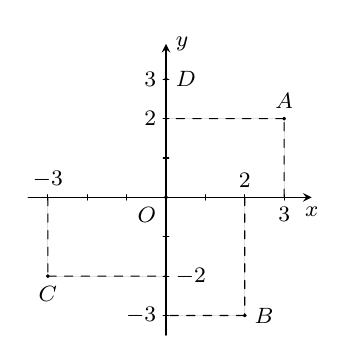
\begin{tikzpicture}[scale=0.5, font=\footnotesize, line join=round, line cap=round,>=stealth]
\def \xmin{-3.5};
\def \xmax{3.7};
\def \ymin{-3.5};
\def \ymax{3.9};
\draw[->] (\xmin, 0.) -- (\xmax,0.) node[anchor=north] {$x$};
\draw[->] (0.,\ymin) -- (0.,\ymax) node[anchor=west] {$y$};
\clip(\xmin,\ymin) rectangle (\xmax,\ymax);
\draw[fill=black, dashed] (3,0) node[below] {$3$} -- (3,2)circle (1pt)node[above]{$A$}--(0,2)node[left] {$2$};
\draw[fill=black, dashed] (2,0) node[above] {$2$} -- (2,-3)circle (1pt)node[right]{$B$}--(0,-3)node[left] {$-3$};
\draw[fill=black, dashed] (-3,0) node[above] {$-3$} -- (-3,-2)circle (1pt)node[below]{$C$}--(0,-2)node[right] {$-2$};
\draw[fill=black, dashed] (0,3) node[left] {$3$} -- (0,3)circle (1pt)node[right]{$D$};
\foreach \x in {-4,-3,-2,-1,1,2,3,4}\draw (\x , 2pt)--(\x , -2pt);
\foreach \y in {-3,-2,-1,1,2,3,4}\draw (2pt, \y) -- (-2pt, \y);
\draw[fill=black] (0,0) circle (1pt) node[below left] {$O$};
\end{tikzpicture}}
	\loigiai
	{Ta có \begin{enumEX}{1}
			\item Điểm $A$ biểu diễn cho số phức $z=3+2i$.
			\item Điểm $B$ biểu diễn cho số phức $z=2-3i$.
			\item Điểm $C$ biểu diễn cho số phức $z=-3-2i$.
			\item Điểm $D$ biểu diễn cho số phức $z=3i$.
		\end{enumEX}		
	}
\end{vd}
\subsubsection{Mô-đun của số phức}
Giả sử số phức $z=a+bi$ được biểu diễn bởi điểm $M(a; b)$ trên mặt phẳng tọa độ.
\immini{\begin{enumEX}{1}
		\item Độ dài của véc-tơ $\overrightarrow{OM}$ được gọi là mô-đun của số phức $z$ và được ký hiệu là $|z|$. Khi đó, $|z|=\left|\overrightarrow{OM}\right|=|a+bi|=\sqrt{a^2+b^2}$.
		\item Kết quả, với mọi số phức $z$ ta có
		\begin{enumerate}
			\item  $|z|\geq 0$ và $|z|=0\Leftrightarrow z=0$.
			\item $z\cdot \bar{z}=|z|^2$.
			\item $|z|=\left|\bar{z}\right|$.
			\item $|z_1\cdot z_2|=|z_1|\cdot |z_2|$.
			\item $\left|\dfrac{z_1}{z_2}\right|=\dfrac{|z_1|}{|z_2|}$.
		\end{enumerate}   
\end{enumEX}}{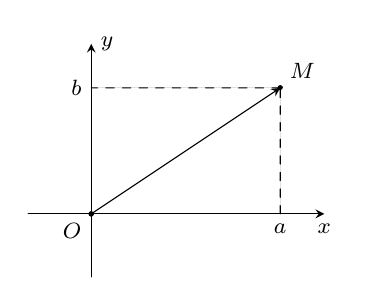
\begin{tikzpicture}[scale=0.8, font=\footnotesize, line join=round, line cap=round,>=stealth]
	\def \xmin{-1.0};
	\def \xmax{3.7};
	\def \ymin{-1.0};
	\def \ymax{2.7};
	\draw[->] (\xmin, 0.) -- (\xmax,0.) node[anchor=north] {$x$};
	\draw[->] (0.,\ymin) -- (0.,\ymax) node[anchor=west] {$y$};
	\clip(\xmin,\ymin) rectangle (\xmax,\ymax);
	\draw[fill=black,dashed] (3,0) node[below] {$a$} -- (3,2)circle (1pt) node[above right]{$M$}--(0,2)node[left] {$b$};
	\draw[->](0,0)--(3,2);
	\draw[fill=black] (0,0) circle (1pt) node[below left] {$O$};
	\end{tikzpicture}}
\begin{vd}%[Lê Hồng Phi, dự án (12-EX-1-DCHT)]%[2D4Y1-1]
	Tìm mô-đun của các số phức sau
	\begin{enumEX}{1}
		\item $z=3-2i\Rightarrow |z|=|3-2i|=\sqrt{\overset{\phantom{3^2+(-2)^2}}{\dots\dots\dots}}=\dots\dots$
		\item $z=1+i\sqrt{3}\Rightarrow |z|=|1+i\sqrt{3}|=\sqrt{\overset{\phantom{1^2+(\sqrt{3})^2}}{\dots\dots\dots}}=\dots\dots$
	\end{enumEX}
	\loigiai
	{Ta có
	\begin{enumEX}{1}
	\item $|z|=|3-2i|=\sqrt{3^2+(-2)^2}=\sqrt{13}$.
	\item $|z|=|1+i\sqrt{3}|=\sqrt{1^2+(\sqrt{3})^2}=2$.
\end{enumEX}		
	}
\end{vd}
\subsubsection{Số phức liên hợp}
\begin{dn}
	Cho số phức $z=a+bi$, $(a, b\in\mathbb{R})$. Ta gọi $a-bi$ là số phức liên hợp của $z$ và được ký hiệu là $\bar{z}=a-bi$.
\end{dn}
\begin{vd}%[Lê Hồng Phi, dự án (12-EX-1-DCHT)]%[2D4Y1-1]\noindent
	\begin{enumEX}{1}
		\item Cho $z=-3-2i\Rightarrow \bar{z}=\dots\dots\dots$
		\item Cho $\bar{z}=4+3i\Rightarrow z=\dots\dots\dots$
	\end{enumEX}
	\loigiai
	{	\begin{enumEX}{1}
			\item Cho $z=-3-2i\Rightarrow \bar{z}=-3+2i$.
			\item Cho $\bar{z}=4+3i\Rightarrow z=4-3i$.
	\end{enumEX}
		
	}
\end{vd}
\immini{\begin{itemize}
		\item Trên mặt phẳng tọa độ, các điểm biểu diễn $z$ và $\bar{z}$ đối xứng với nhau qua trục $Ox$.
		\item Từ định nghĩa ta có các kết quả sau
		\begin{enumerate}[2]
			\item $\bar{\bar{z}}=z$; $\left|\bar{z}\right|=|z|$.
			\item $\overline{z_1\pm z_2}=\bar{z}_1\pm \bar{z}_2$.
			\item $\overline{z_1\cdot z_2}=\bar{z}_1\cdot\bar{z}_2$.
			\item $\overline{\left(\dfrac{z_1}{z_2}\right)}=\dfrac{\bar{z}_1}{\bar{z}_2}$.
			\item $z$ là số thực $\Leftrightarrow z=\bar{z}$.
			\item $z$ là số thuần ảo  $\Leftrightarrow z=-\bar{z}$.
		\end{enumerate}
	\end{itemize}}{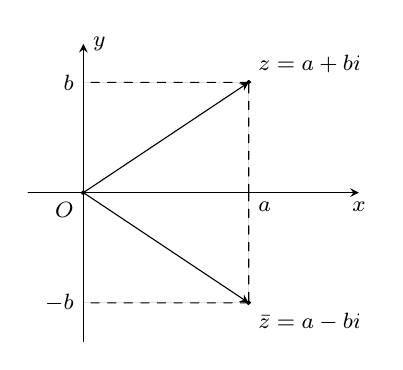
\begin{tikzpicture}[scale=0.7, font=\footnotesize, line join=round, line cap=round,>=stealth]
\def \xmin{-1.0};
\def \xmax{5};
\def \ymin{-2.7};
\def \ymax{2.7};
\draw[->] (\xmin, 0.) -- (\xmax,0.) node[anchor=north] {$x$};
\draw[->] (0.,\ymin) -- (0.,\ymax) node[anchor=west] {$y$};
\clip(\xmin,\ymin) rectangle (\xmax,\ymax);
\draw[fill=black,dashed] (3,0) node[below right] {$a$} -- (3,2)circle (1pt) node[above right]{$z=a+bi$}--(0,2)node[left] {$b$};
\draw[fill=black,dashed] (3,0) -- (3,-2)circle (1pt) node[below right]{$\bar{z}=a-bi$}--(0,-2)node[left] {$-b$};
\draw[->](0,0)--(3,2);
\draw[->](0,0)--(3,-2);
\draw[fill=black] (0,0) circle (1pt) node[below left] {$O$};
\end{tikzpicture}}
\subsubsection{Cộng, trừ, nhân, chia số phức}
Cho hai số phức $z_1=a+bi$ và $z_2=c+di$.
\begin{enumEX}{1}
	\item Phép cộng và phép trừ hai số phức được thực hiện theo quy tắc cộng, trừ đa thức.
	\begin{itemize}
		\item {\bf Phép cộng:} $z_1+z_2=(a+bi)+(c+di)=(a+c)+(b+d)i$.
		\item {\bf Phép trừ:} $z_1-z_2=(a+bi)-(c+di)=(a-c)+(b-d)i$.
		\item Số phức đối của của số phức $z=a+bi$ là $-z=-a-bi$. Do đó, $z+(-z)=(-z)+z=0$.
	\end{itemize}	
\item Phép nhân số phức được thực hiện theo quy tắc nhân đa thức, rồi thay $i^2=-1$	trong kết quả nhận được. Cụ thể, $z_1\cdot z_2=(ac-bd)+(ad+bc)i$.
\item {\bf Phép chia:} $\dfrac{z_1}{z_2}=\dfrac{z_1\cdot\bar{z}_2}{z_2\bar{z}_2}=\dfrac{z_1\cdot\bar{z}_2}{\left|z_2\right|^2}=\dfrac{ac+bd}{c^2+d^2}+\dfrac{bc-ad}{c^2+d^2}\cdot i$, $\left(z_2\neq 0\right)$.
\item Số phức nghịch đảo của $z=a+bi\neq 0$ là $\dfrac{1}{z}=\dfrac{\bar{z}}{|z|^2}=\dfrac{\bar{z}}{a^2+b^2}=\dfrac{a-bi}{a^2+b^2}$.

\end{enumEX}
\end{tomtat}
\subsection{DẠNG TOÁN VÀ BÀI TẬP}
\begin{dang}{Bài toán quy về giải phương trình, hệ phương trình nghiệm thực}
	Phương pháp giải.
Hai số phức là bằng nhau nếu phần thực và phần ảo của chúng tương ứng bằng nhau.
$$a+bi=c+di\Leftrightarrow\heva{& a=c \\ & b=d },\quad \text{với}\ a, b, c, d\in\mathbb{R}.$$
\begin{itemize}
	\item Biểu diễn số phức cần tìm $z=a+bi$ với $a,b\in \mathbb{R}$. Biến đổi thu gọn phương trình của bài toán về dạng $A+Bi=C+Di$.
	\item Giải hệ phương trình $\heva{& A=C \\ & B=D. }$
\end{itemize}
\end{dang}
\subsubsection{Ví dụ}
\begin{vd}%[Lê Hồng Phi, dự án (12-EX-1-DCHT)]%[2D4B2-3]
Tìm các số thực $x$ và $y$ thỏa các điều kiện sau
	\begin{enumEX}{1}
		\item $2x+1+(1-2y)i=2(2-i)+yi-x$. \dapso{$x=1, y=1$}
		\item $(1-2i)x+(1+2y)i=1+i$.  \dapso{$x=1, y=1$}
	\end{enumEX}
\loigiai{
	\begin{enumEX}{1}
		\item Ta có $\begin{aligned}[t]
		2x+1+(1-2y)i=2(2-i)+yi-x &	\Leftrightarrow 	2x+1 +(1-2y)i=4-x+(y-2)i\\
		&\Leftrightarrow  \heva{& 2x+1=4-x \\ & 1-2y=y-2} \Leftrightarrow \heva{& x=1 \\ & y=1. }
	\end{aligned} $\\
	Vậy $x=1, y=1$.
		\item Ta có $(1-2i)x+(1+2y)i=1+i\Leftrightarrow  x +(-2x+1+2y)i=1+i
		\Leftrightarrow  \heva{& x=1 \\ & -2x+1+2y=1 }\Leftrightarrow \heva{& x=1 \\ & y=1. }
		$\\
	Vậy $x=1, y=1$.		
	\end{enumEX}
}
\end{vd}

\begin{vd} %[Nguyễn Quang Tân, dự án (12-EX-1-DCHT)]%[2D4B2-3]
	Tìm số phức $z$ thỏa mãn điều kiện bên dưới. Từ đó xác định phần thực, phần ảo, số phức liên hợp và mô-đun của $z$.
	\begin{enumEX}{1}
		\item  $ \left( 2 + 3i \right)z - \left( 1 + 2i \right)\overline{z} = 7 - i.$
		\dapso{$z=2-i$}
		\item 	% ý 13
		$\left| z - \left( 2 + i \right)\right| = \sqrt{10}$ và $z \cdot \overline{z} = 25$.
		\dapso{$ z = 3 + 4i, z = 5$}
	\end{enumEX}
	\loigiai
	{\begin{enumEX}{1}
			\item	Gọi $z = a + bi \Rightarrow \overline{z} = a - bi, \left(a, b \in \mathbb{R}\right)$.  Ta có
			\begin{eqnarray*}
				&	& \left( 2 + 3i \right) \left( a + bi \right) - \left( 1 + 2i \right)\left( a - bi \right) = 7 - i \\
				&	\Leftrightarrow  &2a + 2bi + 3ai + 3bi^2 - a + bi - 2ai +2bi^2 = 7 - i \\ 
				&	\Leftrightarrow & \left( a - 5b \right) + \left( a+ 3b \right)i = 7 - i \\
				& \Leftrightarrow & \heva{& a - 5b = 7\\& a + 3b = -1 } \Leftrightarrow  \heva{& a = 2\\& b = -1 .} 
			\end{eqnarray*} 
			Suy ra $z = 2 - i \Rightarrow \left| z \right| = \left| 2 - i \right| = \sqrt{ 2^2 + \left( - 1 \right)^2} = \sqrt{5}$. \\
			Vậy phần thực của số phức $z$ là $2$, phần ảo bằng $-1$, số phức liên hợp $\overline{z} = 2 + i$.
			\begin{nx}
				Khi bài toán yêu cầu tìm các thuộc tính của số phức (phần thực, phần ảo,
				mô-đun hoặc số phức liên hợp) mà đề bài cho giả thiết chứa hai thành phần trong ba
				thành phần $z, \overline{z}, \left| z \right|$ thì ta sẽ gọi số phức $z = a + bi \Rightarrow \overline{z} = a - bi, \left| z \right| = \sqrt{a^2 + b^2}$ với $a, b \in \mathbb{R}$, rồi sau đó thu gọn và sử dụng kết quả hai số phức bằng nhau, giải hệ.
			\end{nx} 
			\item Gọi $z = a + bi, \left(a, b \in \mathbb{R}\right)$. Ta có \\ $\left| a + bi - 2 -i \right| = \sqrt{10} \Leftrightarrow \sqrt{\left( a - 2\right)^2 + \left( b - 1 \right)^2 } = \sqrt{10} \Leftrightarrow \left( a - 2 \right)^2 + \left( b - 1\right)^2 = 10$. $\hfill{(1)}$\\
			Lại có $a^2 + b^2 = 25 \Leftrightarrow \left( a - 2 \right)^2 + \left( b - 1\right)^2 + 4a + 2b = 30$. $\hfill{(2)}$ \\ 
			Thế $(1)$ vào $(2)$ ta được $b = 10 - 2a$. Khi đó $a^2 + \left( 10 - 2a \right)^2 = 25 \Leftrightarrow 5a^2 - 40a + 75 = 0 \Rightarrow \hoac{& a = 3 \\ & a = 5.}$ \\
			Với $a = 3 \Rightarrow b = 4.$ \\
			Với $a = 5 \Rightarrow b = 0.$\\
			Vậy có 2 số phức $z$ thỏa mãn đề bài là $z = 3 + 4i$ và $z = 5$.
	\end{enumEX}}
\end{vd}
\begin{vd}%[Nguyễn Quang Tân, dự án (12-EX-1-DCHT)]%[Đề thi THPT Quốc Gia năm 2017 - Mã đề 102 câu 44]%[2D4K2-3] 
	Có bao nhiêu số phức $z$ thỏa mãn $\left| z + 2 - i  \right| = 2 \sqrt{2}$ và $\left( z - 1 \right)^2$ là số thuần ảo?\\
	\quad	\dapso{ $\hoac{& z = -i \\ & z = - 1 + \sqrt{3} + \left( 2 - \sqrt{3} \right)i \\ & z = - 1 - \sqrt{3} + \left( 2 + \sqrt{3} \right)i }$}
	\loigiai{Gọi $z = a + bi,\  \left( a, b \in \mathbb{R}\right).$ \\
		Ta có 
		\begin{eqnarray*}
			& &\left( z - 1 \right)^2 = z^2 - 2z + 1 = \left( a + bi \right)^2 - 2 \left( a + bi \right) + 1\\
			& \Rightarrow &\left( z - 1 \right)^2 = a^2 + 2abi + b^2i^2 - 2a - 2bi + 1 = \left( a^2 - b^2 - 2a + 1 \right) + \left( 2ab - 2b \right)i.
		\end{eqnarray*}
		Vì $\left( z - 1 \right)^2$ là số thuần ảo nên phần thực của nó bằng 0, nghĩa là có $a^2 - b^2 - 2a + 1 = 0 \Leftrightarrow \left( a - 2 \right)^2 - b^2 = 0. \hfill{(1)}$ \\
		Ta có $\left| z + 2 - i \right| = 2 \sqrt{2} \Leftrightarrow \left| a + bi + 2 - i \right| = 2 \sqrt{2} \Leftrightarrow \left| \left( a + 2 \right) + \left( b - 1 \right)i \right| = 2 \sqrt{2} \Leftrightarrow \left( a + 2 \right)^2 + \left( b - 1 \right)^2 = 8. \hfill{(2)} $ \\
		Từ $(1)$ và $(2)$ ta có hệ phương trình 
		\[\heva{& b^2 = \left( a -1 \right)^2 \\ & \left( a + 2 \right)^2 + \left( b - 1 \right)^2 = 8} \Leftrightarrow \hoac{& \heva{& b = a - 1 \\ &\left( a + 2 \right)^2 + \left( b - 1 \right)^2 = 8 }\\ & \heva{& b = 1 - a \\ & \left( a + 2 \right)^2 + \left( b - 1 \right)^2 = 8}} \Leftrightarrow \hoac{& \heva{& b = a - 1 \\ & 2a^2 = 0 }\\ & \heva{& b = 1 - a \\ & a^2 + 2a - 2 = 0}} \Leftrightarrow \hoac{& \heva{& a = 0 \\ & b = -1  }\\ & \heva{& a = - 1 + \sqrt{3} \\ & b = 2 - \sqrt{3}} \\ & \heva{& a = - 1 - \sqrt{3} \\ & b = 2 + \sqrt{3}.}}\]
		Vậy có ba số phức thỏa mãn yêu cầu bài toán là $z = -i, z = - 1 + \sqrt{3} + \left( 2 - \sqrt{3} \right)i, z = - 1 - \sqrt{3} + \left( 2 + \sqrt{3} \right)i$. 
		\begin{nx}
			Số phức $z = a + bi$ được gọi là số phức thuần ảo $\Leftrightarrow$ phần thực $a = 0$ và $z$ là số thực $\Leftrightarrow$ phần ảo $b = 0$. 
	\end{nx}}
\end{vd}
\subsubsection{Bài tập áp dụng}
\begin{ex}%[2D4Y1-1]
Trong các số phức $\left\{z_{1}=3-2 i ;\, z_{2}=1 ;\,z_{3}=4 i ;\,z_{4}=0 ;\,z_{5}=-5 i\right\}$. Có bao nhiêu số phức thuần ảo ?
\choice
{\True $3$}
{$2$}
{$1$}
{$4$}
\loigiai{
Số phức $z=a+bi$ là số thuần ảo khi và chỉ khi $a=0$.\\Vậy $z_3,\,z_4,\,z_5$ là là số thuần ảo.
}
\end{ex}

%%==========Câu 2
\begin{ex}%[2D4Y1-1]
Số phức $z=0$ là số phức
\choice
{Thuần thực}
{Thuần ảo}
{\True Vừa thuần thực vừa thuần ảo}
{không thuần thực cũng không thuần ảo}
\loigiai{
Ta có $z=0=0+0i=a+bi$ nên $\heva{&a=0\Rightarrow z\textrm{ là số thuần ảo}\\&b=0\Rightarrow z\textrm{ là số thuần thực}.}$\\Vậy $z$ vừa thuần thực vừa thuần ảo.
}
\end{ex}

%%==========Câu 3
\begin{ex}%[2D4B1-1]
Cho tập $S$ gồm $6$ số phức, trong đó có $3$ số phức thuần ảo và $4$ số phức thuần thực. Tích tất cả các số phức trong tập $S$ có giá trị bằng
\choice
{$3-2 i$}
{$4+i$}
{$6+6 i$}
{\True$0$}
\loigiai{
Tập có $6$ phần tử mà có tới $3$ số phức thuần ảo và $4$ số phức thuần thực.\\Như vậy, bắt buộc tập $S$ phải chứa số $0$.\\Suy ra tích tất cả các phần tử của tập $S$ bằng $0$.
}
\end{ex}

%%==========Câu 4
\begin{ex}%[2D4Y1-1]
Cho số phức $z=4-2 i$. Phần ảo của số phức là
\choice
{$-2 i$}
{\True $-2$}
{$2 i$}
{$i$}
\loigiai{
Số phức $z=4-2i$ có phần ảo $b=-2$.
}
\end{ex}

%%==========Câu 5
\begin{ex}%[2D4Y1-1]
Cho số phức $z=-1+2 i$. Số phức liên hợp $\bar{z}$ tương ứng là
\choice
{\True $-1-2 i$}
{$1-2 i$}
{$1+2 i$}
{$3 i-2$}
\loigiai{
Ta có $z=-1+2i$ nên số phức liên hợp $\bar{z}=-1-2i$.
}
\end{ex}

%%==========Câu 6
\begin{ex}%[2D4B2-2]
Cho số phức $z=3+4 i$. Số phức liên hợp của số phức $i z$ tương ứng là
\choice
{$-4+3 i$}
{$3-4 i$}
{$3+4 i$}
{\True $-4-3 i$}
\loigiai{
Ta có $z=3+4i$ nên $iz=-4+3i$.\\Khi đó số phức liên hợp $\overline{iz}=-4-3i$.
}
\end{ex}

%%==========Câu 7
\begin{ex}%[2D4B2-1]
Cho số phức $z=(1+i)^{10}$ có phần thực tương ứng là
\choice
{\True $0$}
{$32$}
{$32i$}
{$2$}
\loigiai{
Ta có $(1+i)^2=2i$ nên $(1+2i)^{10}=(2i)^5=32i$.\\Vậy phần thực của $z$ bằng $0$.
}
\end{ex}

%%==========Câu 8
\begin{ex}%[2D4Y1-2]
Trong mặt phẳng phức điểm $M(4 ;-3)$ biểu diễn số phức nào dưới đây ?
\choice
{$z=-(4-3 i)$}
{$z=4 i-3$}
{\True$z=4-3 i$}
{$z=-4+3 i$}
\loigiai{
Điểm $M(4;-3)$ biểu diễn số phức $z=4-3i$.
}
\end{ex}

%%==========Câu 9
\begin{ex}%[2D4Y1-2]
Trong mặt phẳng phức, điểm nào dưới đây biểu diễn đúng số phức $z=-2+3 i$ ?
\choice
{\begin{tikzpicture}[>=stealth,x=1cm,y=1cm,scale=1]
	%	\draw[color=gray,dash pattern=on 1pt off 1pt,xstep=1.0cm,ystep=1.0cm] (-5.2,-5.2) grid (5.2,5.2);
	\draw[->] (-.5,0) -- (2.5,0) node[below] {\scriptsize $x$};
	\draw[->] (0,-.5) -- (0,3.5) node[left] {\scriptsize $y$};
	\draw (0,0)node[below left]{\scriptsize $O$};
	%	\clip (-5,-5)rectangle(5,5);
	\coordinate[label=above right:\scriptsize $A$](A) at (2,3);
	\draw[dashed] (2,0)node[below]{\scriptsize $2$}--(2,3)--(0,3)node[left]{\scriptsize $3$} ;
	\fill[black] (A) circle (1.5pt);
	\end{tikzpicture}}
{\begin{tikzpicture}[>=stealth,x=1cm,y=1cm,scale=1]
	%	\draw[color=gray,dash pattern=on 1pt off 1pt,xstep=1.0cm,ystep=1.0cm] (-5.2,-5.2) grid (5.2,5.2);
	\draw[->] (-.5,0) -- (2.5,0) node[below] {\scriptsize $x$};
	\draw[->] (0,-3.5) -- (0,.5) node[left] {\scriptsize $y$};
	\draw (0,0)node[below left]{\scriptsize $O$};
	%	\clip (-5,-5)rectangle(5,5);
	\coordinate[label=below right:\scriptsize $B$](B) at (2,-3);
	\draw[dashed] (2,0)node[above]{\scriptsize $2$}--(2,-3)--(0,-3)node[left]{\scriptsize $-3$} ;
	\fill[black] (B) circle (1.5pt);
	\end{tikzpicture}}
{\begin{tikzpicture}[>=stealth,x=1cm,y=1cm,scale=1]
	%	\draw[color=gray,dash pattern=on 1pt off 1pt,xstep=1.0cm,ystep=1.0cm] (-5.2,-5.2) grid (5.2,5.2);
	\draw[->] (-3.5,0) -- (.5,0) node[below] {\scriptsize $x$};
	\draw[->] (0,-.5) -- (0,2.5) node[left] {\scriptsize $y$};
	\draw (0,0)node[below left]{\scriptsize $O$};
	%	\clip (-5,-5)rectangle(5,5);
	\coordinate[label=above left:\scriptsize $C$](C) at (-3,2);
	\draw[dashed] (-3,0)node[below]{\scriptsize $-3$}--(-3,2)--(0,2)node[right]{\scriptsize $2$} ;
	\fill[black] (C) circle (1.5pt);
	\end{tikzpicture}}
{\True \begin{tikzpicture}[>=stealth,x=1cm,y=1cm,scale=1]
	%	\draw[color=gray,dash pattern=on 1pt off 1pt,xstep=1.0cm,ystep=1.0cm] (-5.2,-5.2) grid (5.2,5.2);
	\draw[->] (-2.5,0) -- (.5,0) node[below] {\scriptsize $x$};
	\draw[->] (0,-.5) -- (0,3.5) node[left] {\scriptsize $y$};
	\draw (0,0)node[below left]{\scriptsize $O$};
	%	\clip (-5,-5)rectangle(5,5);
	\coordinate[label=above left:\scriptsize $D$](D) at (-2,3);
	\draw[dashed] (-2,0)node[below]{\scriptsize $-2$}--(-2,3)--(0,3)node[right]{\scriptsize $3$} ;
	\fill[black] (D) circle (1.5pt);
	\end{tikzpicture}}
\loigiai{
Số phức $z=-2+3i$ có điểm biểu diễn là $M(-2;3)$.
}
\end{ex}

%%==========Câu 10
\begin{ex}%[2D4Y1-1]
	Cho số phức $z=4-3 i$ mô-đun của nó tương ứng là
	\choice
	{$|z|=1$}
	{$|z|=25$}
	{\True$|z|=5$}
	{$|z|=\sqrt{5}$}
	\loigiai{
		Ta có $z=\sqrt{4^2+(-3)^2}=5$.
	}
\end{ex}

%%==========Câu 11
\begin{ex}%[2D4B1-2]
	\immini{
		Trong mặt phẳng phức, cho $z=1+i$ điểm nào dưới đây biểu diễn đúng số phức $iz$?
		\choice
		{\True Điểm $A$}
		{Điểm $B$}
		{Điểm $C$}
		{Điểm $D$}
	}{
		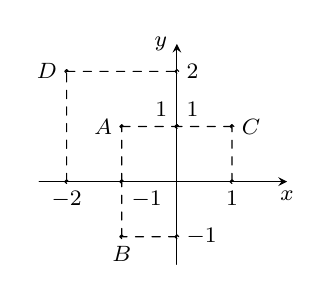
\begin{tikzpicture}[scale=.7,font=\footnotesize,line cap=round,line join=round,>=stealth]
		\draw[->] (-2.5,0)--(2,0)node[below]{$x$};
		\draw[->] (0,-1.5)--(0,2.5)node[left]{$y$};
		\draw[dashed] (-1,0)node[below right]{$-1$}circle(1pt)--(-1,1)node[left]{$A$}circle(1pt)--(0,1)node[above left]{$1$}circle(1pt);
		\draw[dashed] (0,-1)node[right]{$-1$}circle(1pt)--(-1,-1)node[below]{$B$}circle(1pt)--(-1,0);
		\draw[dashed] (1,0)node[below]{$1$}circle(1pt)--(1,1)node[right]{$C$}circle(1pt)--(0,1)node[above right]{$1$}circle(1pt);
		\draw[dashed] (-2,0)node[below]{$-2$}circle(1pt)--(-2,2)node[left]{$D$}circle(1pt)--(0,2)node[right]{$2$}circle(1pt);
		\end{tikzpicture}
	}
	\loigiai{
		Ta có $iz=i(1+i)=i+i^2=-1+i$.
	}
\end{ex}

%%==========Câu 12
\begin{ex}%[2D4B1-1]
	Cho số phức $z$ thỏa mãn $z \cdot\bar{z}=16$ giá trị của $|z|$ tương ứng bằng
	\choice
	{$16$}
	{\True $4$}
	{$\pm4$}
	{$2$}
	\loigiai{
		Ta có $z \cdot\bar{z}=16\Leftrightarrow|z|^2=16\Leftrightarrow z=4$.
	}
\end{ex}

%%==========Câu 13
\begin{ex}%[2D4B1-1]
	Cho số phức $z$ thỏa mãn $\left|z^{3}\right|=0$, số phức $z$ tương ứng là
	\choice
	{$-i$}
	{\True$0$}
	{$i$}
	{$1-i$}
	\loigiai{
		Ta có $\left|z^{3}\right|=0\Leftrightarrow |z|^3=0\Leftrightarrow|z|=0\Leftrightarrow z=0$.
	}
\end{ex}

%%==========Câu 14
\begin{ex}%[2D4B2-2]
	Cho số phức $z$ hệ thức nào dưới đây là \textbf{sai} ?
	\choice
	{$|z|=|\bar{z}|$}
	{$\left|z^{n}\right|=|z|^{n}$}
	{$z \cdot \bar{z}=|z|^{2}$}
	{\True $|z+\bar{z}|=2|z|$}
	\loigiai{
		Hệ thức sai là $|z+\bar{z}|=2|z|$, vì giả sử $z=a+bi$ thì $|z+\bar{z}|=2|a|$.
	}
\end{ex}

%%==========Câu 15
\begin{ex}%[2D4B2-2]
	Cho hai số phức $z_{1},\, z_{2}$   hệ thức nào dưới đây là \textbf{sai} ?
	\choice
	{$\overline{z_{1} \pm z_{2}}=\overline{z_{1}} \pm \overline{z_{2}}$}
	{$\overline{\left(\dfrac{z_{1}}{z_{2}}\right)}=\dfrac{\overline{z_{1}}}{\overline{z_{2}}}$}
	{$\overline{z_{1} \cdot z_{2}}=\overline{z_{1}} \cdot \overline{z_{2}}$}
	{\True $\overline{z_{1}^{2}}=-\left(\overline{z_{1}}\right)^{2}$}
	\loigiai{
		Hệ thức sai là $\overline{z_{1}^{2}}=-\left(\overline{z_{1}}\right)^{2}$, vì $\overline{z_1^2}=\overline{z_1\cdot z_1}=\overline{z_1}\cdot\overline{z_1}=\left(\overline{z_1}\right)^2$.
	}
\end{ex}

%%==========Câu 16
\begin{ex}%[2D4B3-2]
	Cho hai số phức $z_{1},\, z_{2}$ hệ thức nào dưới đây là \textbf{sai} ?
	\choice
	{$\left|z_{1} \cdot z_{2}\right|=\left|z_{1}\right| \cdot\left|z_{2}\right|$}
	{$\left|\dfrac{z_{1}}{z_{2}}\right|=\dfrac{\left|z_{1}\right|}{\left|z_{2}\right|}$ nếu $z_{2} \neq 0$}
	{\True $\left|z_{1} \pm z_{2}\right|=\left|z_{1}\right| \pm\left|z_{2}\right|$}
	{$\left|z_{1}^{n}\right|=\left|z_{1}\right|^{n}$}
	\loigiai{
		Hệ thức sai là $\left|z_{1} \pm z_{2}\right|=\left|z_{1}\right| \pm\left|z_{2}\right|$.
	}
\end{ex}

%%==========Câu 17
\begin{ex}%[2D4Y2-1]
	Phần thực của số phức $(1+i)^{2019}$ tương ứng là
	\choice
	{\True$-2^{1009}$}
	{$2^{1009}$}
	{$0$}
	{$2^{2019}$}
	\loigiai{
		Ta có $(1+i)^{2}=2 i$ nên 
		\begin{eqnarray*}
			(1+i)^{2019}&=&\left((1+i)^{2}\right)^{1009} \cdot(1+i)\\&=&(2 i)^{1009} \cdot(1+i)\\&=&2^{1009} \cdot i^{1009}(1+i)\\&=&2^{1009} \cdot i(1+i)\\&=&2^{1009}(-1+i).
		\end{eqnarray*}
		Suy ra phần thực của số phức $(1+i)^{2019}$ là $-2^{1009}$.
	}
\end{ex}

%%==========Câu 18
\begin{ex}%[2D4Y2-1]
	Phần ảo của số phức $(1-i)^{2020}$ tương ứng là
	\choice
	{$-2^{1010}$}
	{$2^{1010}$}
	{$0$}
	{$-2^{2020}$}
	\loigiai{
		Ta có $(1-i)^{2}=-2 i \Rightarrow(1-i)^{2020}=\left((1+i)^{2}\right)^{1010}=(-2 i)^{1010}=-2^{1010}$.\\
		Suy ra phần ảo của số phức $(1-i)^{2020}$ là $-2^{1009}$.
	}
\end{ex}
\begin{ex}% [2D4K1-1]%[TheHung Nguyen]	
Phần ảo của số phức $(1+i\sqrt 3)^{2021}$ tương ứng là
	\choice
	{$2^{2020}\cdot\sqrt 3$}
	{\True $-2^{2020}\cdot\sqrt 3$}
	{$-2^{2020}$}
	{$2^{2020}$}
	\loigiai{
\begin{enumerate}[•]
	\item Ta có $(1+i\sqrt 3)^3=1+3i\sqrt 3+3\cdot(i\sqrt 3)^2+(i\sqrt 3)^3=-8$.
	\item Khi đó $(1+i\sqrt 3)^{2021}=\left((1+i\sqrt 3)^3\right)^{673}\cdot(1+i\sqrt 3)^2=(-8)^{673}\cdot(-2+2i\sqrt 3)=2^{2020}(1-i\sqrt 3)$.
	\item Vậy phần ảo của số phức 	$(1+i\sqrt 3)^{2021}$ là $-2^{2020}\cdot\sqrt 3$.
\end{enumerate}		
	}
\end{ex}

%20
\begin{ex}% [2D4K1-1]%[TheHung Nguyen]	
Phần thực của số phức $\dfrac{(1-i\sqrt 3)^{2021}}{(1-i)^{2021}}$ tương ứng là 
	\choice
	{$2^{1009}(\sqrt 3+1)$}
	{$2^{1009}$}
	{\True $2^{1009}(\sqrt 3-1)$}
	{$2^{1009}(1-\sqrt 3)$}
	\loigiai{
\begin{enumerate}[•]
	\item	Ta có $(1-i\sqrt 3)^3=1-3i\sqrt 3+3\cdot(i\sqrt 3)^2-(i\sqrt 3)^3=-8$.
	\item Khi đó $(1-i\sqrt 3)^{2021}=\left((1-i\sqrt 3)^3\right)^{673}\cdot(1-i\sqrt 3)^2=(-8)^{673}\cdot(-2-2i\sqrt 3)=2^{2020}(1+i\sqrt 3)$.
	\item Ta có $(1-i)^2=-2i$.
	\item Khi đó  $(1-i)^{2021}=\left((1-i)^2\right)^{1010}\cdot(1-i)=(-2i)^{1010}\cdot(1-i)=-2^{1010}(1-i)$.
	\item Vậy $\dfrac{(1-i\sqrt 3)^{2021}}{(1-i)^{2021}}=\dfrac{2^{2020}(1+i\sqrt 3)}{-2^{1010}(1-i)}=2^{1010}\cdot\dfrac{1+i\sqrt 3}{i-1}=2^{1010}\left(\dfrac{-1+\sqrt 3}2+\dfrac{-1-\sqrt 3}2i\right)$.
	\item Suy ra Phần thực của số phức $\dfrac{(1-i\sqrt 3)^{2021}}{(1-i)^{2021}}$ là $2^{1009}(\sqrt 3-1)$.
\end{enumerate}
	}
\end{ex}

%21
\begin{ex}%[2D4K1-2]%[TheHung Nguyen]	
	Cho số phức $z$ biểu diễn điểm $M$ trên mặt phẳng $Oxy$. Hỏi điểm nào dưới đây biểu diễn đúng số phức $\dfrac{1}{z}$.
	\begin{center}
	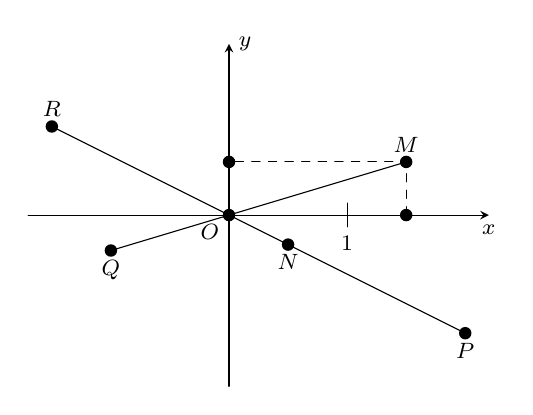
\begin{tikzpicture}[scale=1.5, font=\footnotesize, line join=round, line cap=round, >=stealth]
	\def\xmin{-1.5}\def\xmax{2}\def\ymin{-1.25}\def\ymax{1.25}
	\draw[->] (\xmin-0.2,0)--(\xmax+0.2,0) node[below] {\footnotesize $x$};
	\draw[->] (0,\ymin-0.2)--(0,\ymax+0.2) node[right] {$y$};
	\draw (0,0) node [below left] {$O$};
	\foreach \x in {1}\draw (\x,0.1)--(\x,-0.1) node [below] {\footnotesize $\x$};
	\foreach \y in {}\draw (0.1,\y)--(-0.1,\y) node [left] {\footnotesize $\y$};
	
	\draw[dashed] (1.5,0)--(1.5,.45) node[above] {$M$}--(0,.45);
	
	\draw (1.5,.45)--(-1,-.3)node[below] {$Q$}
	(2,-1)node[below] {$P$}--(.5,-.25)node[below] {$N$}--(-1.5,.75)node[above] {$R$}
	;
	\foreach \a in {(1.5,0),(1.5,.45),(0,.45),(0,0),(-1,-.3),(2,-1),(-1.5,.75),(.5,-.25)}
	\fill \a circle (1.5pt);
	\end{tikzpicture}
	\end{center}
	\choice
	{$P$}
	{\True $N$}
	{$Q$}
	{$R$}
	\loigiai{
\textbf{Cách 1:} Trắc nghiệm.\\
Ta chọn số phức $z$ bất kỳ hợp lý là $z=1{,}5+0{,}5i\Rightarrow\dfrac 1 z=0{,}6-0{,}2i ;|z|<1$. Suy ra chọn điểm $N$.\\
\textbf{Cách 2:}\\
Ta có $\dfrac 1 z=\dfrac{\bar z}{z \cdot\bar z}=\dfrac{\bar z}{|z|^2}$. Suy ra góc tạo bởi số phức $z$ với trục $Ox$ đối với góc tạo bởi $\dfrac{1}{z}$ và trục $Ox$, đồng thời ta có $|z|>1\Rightarrow\left|\dfrac 1 z\right|<1$. Nên ta chọn điểm $N$.
	}
\end{ex}

%22
\begin{ex}%[2D4K2-1]%[TheHung Nguyen]	
Tổng 	$S=\mathrm{C}_{2019}^0-\mathrm{C}_{2019}^2+\mathrm{C}_{2019}^4-\mathrm{C}_{2019}^6+\ldots-\mathrm{C}_{2019}^{2018}$ có giá trị bằng 
	\choice
	{$2^{1009}$}
	{$-2^{2019}$}
	{$2^{2019}$}
	{\True $-2^{1009}$}
	\loigiai{
	Ta có 
$\begin{aligned}[t]
(1+i)^{2019}=& \mathrm{C}_{2019}^0+\mathrm{C}_{2019}^1\cdot i+\mathrm{C}_{2019}^2\cdot i^2+\mathrm{C}_{2019}^3\cdot i^3+\mathrm{C}_{2019}^4\cdot i^4+\ldots+\mathrm{C}_{2019}^{2018}\cdot i^{2018}+\mathrm{C}_{2019}^{2019}\cdot i^{2019} \\ 
= &~ \left(\mathrm{C}_{2019}^0-\mathrm{C}_{2019}^2+\mathrm{C}_{2019}^4-\mathrm{C}_{2019}^6+\ldots-\mathrm{C}_{2019}^{2018}\right)+i\left(\mathrm{C}_{2019}^1-\mathrm{C}_{2019}^3+\ldots-\mathrm{C}_{2019}^{2019}\right).
\end{aligned}$	
Ta lại có $(1+i)^{2019}=\left((1+i)^2\right)^{1009}(1+i)=(2i)^{1009}\cdot(1+i)=2^{1009}\cdot i(1+i)=2^{1009}(-1+i)$.\\
Do đó $2^{1009}(-1+i)=\left(\mathrm{C}_{2019}^0-\mathrm{C}_{2019}^2+\mathrm{C}_{2019}^4-\mathrm{C}_{2019}^6+\ldots-\mathrm{C}_{2019}^{2018}\right)+i\left(\mathrm{C}_{2019}^1-\mathrm{C}_{2019}^3+\ldots-\mathrm{C}_{2019}^{2019}\right)$.
Suy ra $\left(\mathrm{C}_{2019}^0-\mathrm{C}_{2019}^2+\mathrm{C}_{2019}^4-\mathrm{C}_{2019}^6+\ldots-\mathrm{C}_{2019}^{2018}\right)=-2^{1009}$

	}
\end{ex}

%23
\begin{ex}%[2D4K2-1]%[TheHung Nguyen]	
Tổng $S=\mathrm{C}_{2020}^1-\mathrm{C}_{2020}^3+\mathrm{C}_{2020}^5-\mathrm{C}_{2020}^7+\ldots-\mathrm{C}_{2020}^{2019}$ có giá trị bằng 
	\choice
	{\True $0$}
	{$-2^{1010}$}
	{$2^{2020}$}
	{$2^{1010}$}
	\loigiai{
	Ta có 
$\begin{aligned}[t]
(1+i)^{2019}=& \mathrm{C}_{2020}^0+\mathrm{C}_{2020}^1i+\mathrm{C}_{2020}^2\cdot i^2+\mathrm{C}_{2020}^3\cdot i^3+\mathrm{C}_{2020}^4\cdot i^4+\ldots+\mathrm{C}_{2020}^{2019}\cdot i^{2019}+\mathrm{C}_{2020}^{2020}\cdot i^{2020} \\ 
= &~ \left(\mathrm{C}_{2020}^0-\mathrm{C}_{2020}^2+\mathrm{C}_{2020}^4-\ldots+\mathrm{C}_{2020}^{2020}\right)+i\left(\mathrm{C}_{2020}^1-\mathrm{C}_{2020}^3+\ldots-\mathrm{C}_{2020}^{2019}\right).
\end{aligned}$
Ta lại có $(1+i)^{2020}=\left((1+i)^2\right)^{1010}=(2i)^{1010}=-2^{1010}$.\\
Do đó $-2^{1010}=\left(\mathrm{C}_{2020}^0-\mathrm{C}_{2020}^2+\mathrm{C}_{2020}^4-\ldots+\mathrm{C}_{2020}^{2020}\right)+i\left(\mathrm{C}_{2020}^1-\mathrm{C}_{2020}^3+\ldots-\mathrm{C}_{2019}^{2019}\right)$.\\
Suy ra $\left(\mathrm{C}_{2020}^1-\mathrm{C}_{2020}^3+\ldots-\mathrm{C}_{2019}^{2019}\right)=0$.
	}
\end{ex}

%24
\begin{ex}%[2D4K2-1]%[TheHung Nguyen]	
Tổng $S=\mathrm{C}_{2019}^0-3\mathrm{C}_{2019}^2+3^2\mathrm{C}_{2019}^4-3^3\mathrm{C}_{2019}^6+\ldots-3^{1009}\mathrm{C}_{2019}^{2018}$ có giá trị bằng 	
	\choice
	{$2^{2019}$}
	{$0$}
	{\True $-2^{2019}$}
	{$-2^{1009}$}
	\loigiai{
Ta có\\
$\begin{aligned}
&(1+i\sqrt 3)^{2019}\\
&= \mathrm{C}_{2019}^0+\mathrm{C}_{2019}^1i\sqrt 3+\mathrm{C}_{2019}^2\cdot(i\sqrt 3)^2+\mathrm{C}_{2019}^3\cdot(i\sqrt 3)^3+\mathrm{C}_{2019}^4\cdot(i\sqrt 3)^4+\ldots+\mathrm{C}_{2019}^{2019}\cdot(i\sqrt 3)^{2019}\\ 
= &~ \left(\mathrm{C}_{2019}^0-3\mathrm{C}_{2019}^2+3^2\mathrm{C}_{2019}^4-\ldots-3^{1009}\mathrm{C}_{2019}^{2018}\right)+i\left(\sqrt 3\mathrm{C}_{2019}^1-(\sqrt 3)^3\mathrm{C}_{2019}^3+\ldots-(\sqrt 3)^{2019}\mathrm{C}_{2019}^{2019}\right).
\end{aligned}$
Ta lại có $(1+i\sqrt 3)^{2019}=\left((1+i\sqrt 3)^3\right)^{673}=(-8)^{673}=-2^{2019}$.\\
Do đó $-2^{2019}=\left(\mathrm{C}_{2019}^0-3\mathrm{C}_{2019}^2+3^2\mathrm{C}_{2019}^4-\ldots-3^{1009}\mathrm{C}_{2019}^{2018}\right)\\
+i\left(\sqrt 3\mathrm{C}_{2019}^1-(\sqrt 3)^3\mathrm{C}_{2019}^3+\ldots-(\sqrt 3)^{2019}\mathrm{C}_{2019}^{2019}\right)$.\\
Suy ra $\left(\mathrm{C}_{2019}^0-3\mathrm{C}_{2019}^2+3^2\mathrm{C}_{2019}^4-\ldots-3^{1009}\mathrm{C}_{2019}^{2018}\right)=-2^{2019}$.
	}
\end{ex}




%25
\begin{ex}%[2D4K3-2]%[TheHung Nguyen]	
Cho $f(x)=\dfrac{(x+2)}{(x-1)\left(x^2+1\right)(x+3)}\equiv\dfrac{A}{x-1}+\dfrac{B}{x+3}+\dfrac{C x+D}{x^2+1}$. Giá trị của $C+D$ bằng
	\choice
	{$\dfrac{3}{5}$}
	{$-\dfrac{7}{10}$}
	{$0$}
	{\True $-\dfrac{9}{10}$}
	\loigiai{
	Nhân hai vế với $x^2+1$, ta được $\dfrac{(x+2)}{(x-1)(x+3)}\equiv\left(x^2+1\right)\left(\dfrac{A}{x-1}+\dfrac{B}{x+3}\right)+C x+D$.\\
	Thay $x=i$ vào ta được $\dfrac{(i+2)}{(i-1)(i+3)}\equiv\left(i^2+1\right)\left(\dfrac{A}{x-1}+\dfrac{B}{x+3}\right)+C i+D$.\\
	Do đó ta có $-\dfrac 3{10}-\dfrac 25i\equiv 0+C i+D$. \\
	Suy ra $\heva{&C=-\dfrac 25\\ &D=-\dfrac 3{10}.}$\\
	Vậy $C+D=-\dfrac 7{10}$.
	}
\end{ex}

%26
\begin{ex}%[2D4K3-2]%[TheHung Nguyen]	
Ta có $f(x)=\dfrac{x^3+3}{(x+1)\left(x^2+1\right)\left(x^2+4\right)}\equiv\dfrac{A}{x+1}+\dfrac{B x+C}{x^2+1}+\dfrac{D x+E}{x^2+4}$. Giá trị của biểu thức $(D+E)$ bằng
	\choice
	{\True $\dfrac{4}{3}$}
	{$\dfrac{9}{5}$}
	{$-\dfrac{13}{15}$}
	{$\dfrac{7}{6}$}
	\loigiai{
	Nhân hai vế với $x^2+4$ ta được $\dfrac{x^3+3}{(x+1)\left(x^2+1\right)}\equiv\left(x^2+4\right)\left(\dfrac{A}{x+1}+\dfrac{B x+C}{x^2+1}\right)+D x+E$.\\
	Thay $x=2i$ vào ta được $\dfrac{(2i)^3+3}{(2i+1)\left((2i)^2+1\right)}\equiv\left((2i)^2+4\right)\left(\dfrac{A}{x+1}+\dfrac{B x+C}{x^2+1}\right)+D(2i)+E$.\\
	Do đó $\dfrac{13}{15}+\dfrac{14}{15}i\equiv D(2i)+E$.\\
	Từ đó ta có $\heva{&{2D=\dfrac{1 4}{1 5}}\\ &{E=\dfrac{1 3}{1 5}}}\Leftrightarrow\heva{&D=\dfrac 7{15}\\ &E=\dfrac{13}{15}}\Rightarrow(D+E)=\dfrac 43$.
	}
\end{ex}

%27
\begin{ex}%[2D4B3-2]%[TheHung Nguyen]	
	Cho số phức $z$ thỏa mãn $(1-2i)z=(4+3i)(2-z)$. Giá trị $|z|$ bằng
	\choice
	{$\dfrac 5{\sqrt{13}}$}
	{\True $\dfrac{5\sqrt{26}}{13}$}
	{$2\sqrt 3$}
	{$\dfrac{5\sqrt 5}2$}
	\loigiai{
	Ta có $(1-2i)z=(4+3i)(2-z)\Leftrightarrow z((1-2i)+(4+3i))=2(4+3i)$.\\
	Suy ra $z=\dfrac{2(4+3i)}{(1-2i)+(4+3i)}$.\\
	Vậy $|z|=\left|\dfrac{2(4+3i)}{(1-2i)+(4+3i)}\right|=\dfrac{5\sqrt{26}}{13}$.
	}
\end{ex}

%28
\begin{ex}%[2D4K3-2] %[TheHung Nguyen]	
Cho số phức $z$ khác $0$, thỏa mãn $(1+2i)z^2=(4-3i)\cdot\bar z$. Giá trị $|z|$ bằng
	\choice
	{$\sqrt{5}$}
	{$1$}
	{$2$}
	{$\sqrt{3}$}
	\loigiai{
	Ta có $|1+2i|\cdot\left|z^2\right|=|4-3i|\cdot|\bar z|\Leftrightarrow\sqrt 5\cdot|z|^2=5 \cdot|z|\Leftrightarrow \hoac{& |z|=0 ~~\text{loại vì}~~z=0\\ & |z|=\sqrt{5}.}$ \\
	Suy ra $|z|=\sqrt 5$.	
	}
\end{ex}

%29
\begin{ex}%[2D4K2-3]%[TheHung Nguyen]	
Cho số phức $z$ khác $0$, thỏa mãn $(z+2i)(1-i)=i(3i+\bar z)$. Phần thực của số phức $z$ bằng
	\choice
	{$3\sqrt{5}$}
	{$3$}
	{$2\sqrt{13}$}
	{\True $13$}
	\loigiai{
Gọi $z=a+i b\Rightarrow\bar z=a-i b$.\\
Thay vào phương trình đầu bài ta được 
\begin{eqnarray*}
	&&  (a+i b+2i)(1-i)=i(3i+a-i b) \\
	&\Leftrightarrow& a-i a+i b+b+2i+2=-3+i a+b \\
	&\Leftrightarrow& (a+5)+i(-2a+b+2)=0\\
	&\Leftrightarrow& \heva{&a+5=0\\ &-2a+b+2=0}\\
	&\Leftrightarrow&\heva{&a=-5\\ &b=-12.}
\end{eqnarray*} 
Suy ra $z=-5-12i\Rightarrow|z|=13$.
	}
\end{ex}

%30
\begin{ex}%[2D4K2-2]%[TheHung Nguyen]	
Tổng $S=1+i+i^2+\ldots+i^{2019}$ bằng 
	\choice
	{$1$}
	{$i$}
	{\True $0$}
	{$-i$}
	\loigiai{
	\textbf{Cách 1:} Tổng  liên tiếp $4$ số hạng lũy thừa ảo tăng dần luôn bằng $0$.\\
	Do đó
	\begin{eqnarray*}
		&S=&1+i+i^2+\ldots+i^{2019} \\
		&=& \left(1+i+i^2+i^3\right)+\left(i^4+i^5+i^6+i^7\right)+\ldots+\left(i^{2016}+i^{2017}+i^{2018}+i^{2019}\right) \\
		&=&0.
	\end{eqnarray*}
	\textbf{Cách 2:} Cấp số nhân $S=1+i+i^2+\ldots+i^{2019}=1\cdot\dfrac{i^{2020}-1}{i-1}=0$.
	}
\end{ex}

%31
\begin{ex}%[2D4K2-2]%[TheHung Nguyen]	
Phần thực của số phức $z=1+2i+3i^2+\ldots+2020i^{2019}$ tương ứng bằng 
	\choice
	{$1010$}
	{$2020$}
	{$-2^{1010}$}
	{\True $-1010$}
	\loigiai{
	Ta có $1+x+x^2+\ldots+x^{2020}=\dfrac{x^{2021}-1}{x-1}$.\\
	Đạo hàm hai vế ta được $1+2x+3x^2+\ldots+2020x^{2019}=\dfrac{2021x^{2020}(x-1)-\left(x^{2021}-1\right)}{(x-1)^2}$.\\
	Thay $x=1$ vào ta được $1+2i+3i^2+\ldots+2020i^{2019}=\dfrac{2021\cdot i^{2020}(i-1)-\left(i^{2021}-1\right)}{(i-1)^2}$.\\
	Do đó $z=1+2i+3i^2+\ldots+2020i^{2019}=\dfrac{2021\cdot(i-1)-(i-1)}{-2i}=-1010-1010i$.\\
	Vậy phần thực của số phức $z$ là $-1010$.
	}
\end{ex}

%32
\begin{ex}%[2D4K5-2]%[TheHung Nguyen]	
Cho số phức $z=a+i b$ và $z^2=a_0+i b_0$ với $a>0$. Giá trị lớn nhất của biểu thức $T=\dfrac{a_0+a+1}{a^2+1}$ tương ứng bằng
	\choice
	{$1$}
	{$2$}
	{\True $\dfrac{3}{2}$}
	{$\dfrac{5}{3}$}
	\loigiai{
Ta có $z^2=a_0+i b_0=a^2-b^2+2a b i\Rightarrow a_0=a^2-b^2$.\\
Suy ra $T=\dfrac{a^2-b^2+a+1}{a^2+1}=\dfrac{a^2+a+1}{a^2+1}-\dfrac{-b^2}{a^2+1}\leq\dfrac{a^2+a+1}{a^2+1}=f(a)$.\\
Khảo sát hàm số $f(a)=\dfrac{a^2+a+1}{a^2+1}=1+\dfrac a{a^2+1}=1+\dfrac 1{a+\dfrac 1 a}\leq 1+\dfrac 12=\dfrac 32$.\\
Dấu~ \lq\lq $=$ \rq\rq~ xảy ra khi $a=1 ; b=0$.\\
Vậy giá trị lớn nhất của biểu thức $T$ là $\dfrac{3}{2}$.
	}
\end{ex}

%33
\begin{ex}%[2D4K5-2]%[TheHung Nguyen]	
	Cho số phức $z=a+ib$ và $z^2=a_0+i b_0$ với $ a, b\in\mathbb{R}$. Khi biểu thức $T=\dfrac{a_0-2a+2}{a^2+1}$ đạt giá trị lớn nhất thì môđun của số phức $z$ tương ứng bằng 
	\choice
	{\True $\dfrac{\sqrt 5-1}2$}
	{$\dfrac{\sqrt 5+1}2$}
	{$\dfrac{1+\sqrt 3}2$}
	{$\dfrac{3}{2}$}
	\loigiai{
	Ta có $z^2=a_0+i b_0=a^2-b^2+2a b i\Rightarrow a_0=a^2-b^2$.\\
	Suy ra $T=\dfrac{a^2-b^2-2a+2}{a^2+1}=\dfrac{a^2-2a+2}{a^2+1}-\dfrac{-b^2}{a^2+1}\leq\dfrac{a^2-2a+2}{a^2+1}=f(a)$.\\
	Khảo sát hàm số $f(a)=\dfrac{a^2-2a+2}{a^2+1}; f'(a)=\dfrac{2a^2-2a-2}{\left(a^2+1\right)^2}=0\Leftrightarrow a=\dfrac{1\pm\sqrt 5}2$.\\
	Ta có bảng biến thiên
	\begin{center}
		
\begin{tikzpicture}[>=stealth]
		\tkzTabInit[nocadre=false,lgt=2,espcl=2,deltacl=0.5]{$a$/1 ,$f'(a)$/.7,$f(a)$/2}
		{$-\infty$ , $\tfrac{1-\sqrt 5}2$, $\tfrac{1+\sqrt 5}2$ , $+\infty$}
		\tkzTabLine{ , + , $0$ , - , $0$ , + , }
		\tkzTabVar{-/$1$ , +/$max$ , -/$min$ , +/$1$}
		\end{tikzpicture}		
	\end{center}
Suy ra biểu thức đạt giá trị lớn nhất khi $a=\dfrac{1-\sqrt 5}2$ và $b=0$.\\
Vậy $|z|=\sqrt{a^2+b^2}=\dfrac{\sqrt 5-1}2$.
	}
\end{ex}

%34
\begin{ex}%[2D4K5-2]%[TheHung Nguyen]	
Cho số phức $z=a+ib$ và $z^4=a_0+i b_0$ với $a, b\in\mathbb{R}, a\neq 0$. Giá trị nhỏ nhất của biểu thức $T=\dfrac{a_0}{a^4}$ tương ứng bằng
	\choice
	{$1$}
	{\True $-8$}
	{$3$}
	{$-5$}
	\loigiai{
	Ta có $z^4=a_0+i b_0=\left(a^4-6\cdot a^2b^2+b^4\right)+\left(4a^3b-4a b^3\right)i\Rightarrow a_0=a^4-6\cdot a^2b^2+b^4$.\\
	Suy ra $T=\dfrac{a_0}{a^4}=\dfrac{a^4-6\cdot a^2b^2+b^4}{a^4}=1-6\dfrac{b^2}{a^2}+\dfrac{b^4}{a^4}=\left(\dfrac{b^2}{a^2}-3\right)^2-8\geq-8$.\\
	Dầu \lq\lq ~$=$ \rq\rq~ xảy ra khi $\dfrac{b^2}{a^2}-3=0\Leftrightarrow b=\pm a\sqrt 3$.\\
	Vậy biểu thức đạt giá trị nhỏ nhất bằng $-8$.
	}
\end{ex}


%35
\begin{ex}%[2D4G5-2]%[TheHung Nguyen]	
Cho số phức $z=a+i b$ với $a, b\in\mathbb{R}, b\neq 0,|a|\leq|b|$. Giá trị lớn nhất của biểu thức $T=\left|\dfrac{z^4-\overline{z^4}}{(z-\bar z)^4}\right|$ tương ứng bằng 
	\choice
	{\True $\dfrac 2{3\sqrt 3}$}
	{$1$}
	{$\dfrac 3{\sqrt 2}$}
	{$\sqrt 3$}
	\loigiai{
	Ta có $z^4=\left(a^4-6\cdot a^2b^2+b^4\right)+\left(4a^3b-4a b^3\right)i\Rightarrow\bar z^4=\left(a^4-6\cdot a^2b^2+b^4\right)-\left(4a^3b-4a b^3\right)i$.\\
	Suy ra $\heva{&z^4-\overline{z^4}=2\left(4a^3b-4a b^3\right)i\\ &z-\bar z=2b i.}$\\
	Suy ra $T=\left|\dfrac{z^4-\overline{z^4}}{(z-\bar z)^4}\right|=\left|\dfrac{2\left(4a^3b-4a b^3\right)i}{(2b i)^4}\right|=\dfrac 12\left|\dfrac{a^3b-a b^3}{b^4}\right|=\dfrac 12\left|\left(\dfrac ab\right)^3-\left(\dfrac ab\right)\right|=\dfrac 12|f(t)|$.\\
	Với $f(t)=\left(\dfrac ab\right)^3-\left(\dfrac ab\right)=t^3-t ;-1\leq t=\dfrac ab\leq 1$.\\
	Ta có bảng biến thiên
	\begin{center}
	
\begin{tikzpicture}[>=stealth]
	\tkzTabInit[nocadre=false,lgt=1.5,espcl=2,deltacl=0.5]{$a$/1 ,$f'(a)$/.7,$f(a)$/2}
	{$-1$ , $-\tfrac{1}{\sqrt{3}}$ , $\tfrac{1}{\sqrt{3}}$ , $1$}
	\tkzTabLine{ , + , $0$ , - , $0$ , + , }
	\tkzTabVar{-/$0$ , +/$\tfrac 2{3\sqrt 3}$ , -/$-\tfrac 2{3\sqrt 3}$ , +/$0$}
	\end{tikzpicture}	
	\end{center}
Suy ra giá trị lớn nhất của biểu thức $T$ là $\dfrac{2}{3\sqrt{3}}$.
	}
\end{ex}


\begin{ex}%[2D4B3-2]
Cho số phức $z$ thỏa mãn phương trình $(2-3i)z=5+11i$. Phần thực của số phức $z$ bằng
\choice
{\True $-\dfrac{23}{13}$}
{$\dfrac{37}{13}$}
{$\dfrac{23}{13}$}
{$-\dfrac{23}{146}$}
\loigiai{
Ta có $(2-3i)z=5+11i \Leftrightarrow z=\dfrac{5+11i}{2-3i}=-\dfrac{23}{13}+\dfrac{37}{13}i$.\\
Phần thực của số phức $z$ bằng $-\dfrac{23}{13}$.
}
\end{ex}

%%==========Câu 2
\begin{ex}%[2D4B3-2]
Cho số phức $z$ thỏa mãn phương trình $(1-3i)(z-2i)-(3+i)z+3i=0$. Phần ảo của số phức $z$ bằng
\choice
{$-\dfrac{2}{5}$}
{$\dfrac{11}{10}$}
{$-\dfrac{9}{5}$}
{\True $\dfrac{13}{10}$}
\loigiai{
Ta có $(1-3i)(z-2i)-(3+i)z+3i=0 \Leftrightarrow (-2-4i)z=6-i \Leftrightarrow z=\dfrac{6-i}{-2-4i}=-\dfrac{2}{5}+\dfrac{13}{10}i$.\\
Phần thực của số phức $z$ bằng $\dfrac{13}{10}$.
}
\end{ex}

%%==========Câu 3
\begin{ex}%[2D4B3-2]
Số phức $z$ thỏa mãn điều kiện $z=4+3\overline{z}$ có mô-đun bằng
\choice
{\True $\sqrt{5}$}
{$2$}
{$-2$}
{$4$}
\loigiai{
Đặt $z=a+bi$, $(a;b\in\mathbb{R})$.\\
Ta có $z=4+3\overline{z} \Leftrightarrow \heva{&a=4+3a\\&b=4-3b} \Leftrightarrow \heva{&a=-2\\&b=1.}$\\
Vậy $|z|=\sqrt{(-2)^2+1^2}=\sqrt{5}$.
}
\end{ex}

%%==========Câu 4
\begin{ex}%[2D4B3-3]
Số phức $z$ thỏa mãn điều kiện $z=-3+4\overline{z}$ có mô-đun bằng
\choice
{\True $\dfrac{\sqrt{34}}{5}$}
{$\dfrac{7}{5}$}
{$\dfrac{\sqrt{35}}{5}$}
{$\dfrac{6}{5}$}
\loigiai{
	Đặt $z=a+bi$, $(a;b\in\mathbb{R})$.\\
	Ta có $z=-3+4\overline{z} \Leftrightarrow \heva{&a=-3+4a\\&b=-3-4b} \Leftrightarrow \heva{&a=1\\&b=-\dfrac{3}{5}.}$\\
	Vậy $|z|=\sqrt{1^2+\left(-\dfrac{3}{5}\right)^2}=\dfrac{\sqrt{34}}{5}$.
}
\end{ex}

%%==========Câu 5
\begin{ex}%[2D4B3-2]
Cho số phức $z$ thỏa mãn phương trình $(1+i)(z+2-4i)=(3-2i)(4+5i)$. Giá trị của biểu thức $T=\left|z_1+z_2\right|$ bằng
\choice
{$\dfrac{33}{2}$}
{$\dfrac{\sqrt{1065}}{2}$}
{\True $\dfrac{\sqrt{1066}}{2}$}
{$5\sqrt{7}$}
\loigiai{
Ta có $(1+i)(z+2-4i)=(3-2i)(4+5i) \Leftrightarrow z+2-4i=\dfrac{(3-2i)(4+5i)}{1+i}=\dfrac{29}{2}-\dfrac{15}{2}i$.\\
Suy ra $T=\left|z_1+z_2\right|=\sqrt{\left(\dfrac{29}{2}\right)^2+\left(-\dfrac{15}{2}\right)^2}=\dfrac{\sqrt{1066}}{2}$.
}
\end{ex}

%%==========Câu 6
\begin{ex}%[2D4B3-3]
Cho số phức $z$ thỏa mãn phương trình $i(z-1)+(2-i)\overline{z}=6$. Phần ảo của số phức $z$ bằng
\choice
{$\dfrac{5}{2}$}
{\True $-\dfrac{1}{2}$}
{$-\dfrac{5}{2}$}
{$\dfrac{1}{2}$}
\loigiai{
Đặt $z=a+bi$, $(a;b\in\mathbb{R})$.\\
Ta có
\allowdisplaybreaks
$\begin{aligned}[t]
	&\quad i(z-1)+(2-i)\overline{z}=6 \Leftrightarrow i(a-1+bi)+(2-i)(a-bi)=6\\
	&\Leftrightarrow 2(a-b)+(-2b-1)i=6 \Leftrightarrow \heva{&2a-2b=6\\&-2b-1=0} \Leftrightarrow \heva{&a=\dfrac{5}{2}\\&b=-\dfrac{1}{2}.}
\end{aligned}$\\
Phần ảo của số phức $z$ bằng $-\dfrac{1}{2}$.
}
\end{ex}

%%==========Câu 7
\begin{ex}%[2D4B3-2]
Cho số phức $z$ thỏa mãn phương trình $\overline{iz-3i+4}=\overline{z+1}-2i+3$. Mô-đun của số phức $z$ bằng
\choice
{\True $\dfrac{5}{\sqrt{2}}$}
{$\sqrt{2}$}
{$3$}
{$1$}
\loigiai{
Ta có
\allowdisplaybreaks
$\begin{aligned}[t]
	&\quad \overline{iz-3i+4}=\overline{z+1}-2i+3 \Leftrightarrow iz-3i+4=z+1+2i+3\\
	&\Leftrightarrow (1-i)z=-5i \Leftrightarrow z=\dfrac{-5i}{1-i}=\dfrac{5}{2}-\dfrac{5}{2}i
\end{aligned}$\\
Mô-đun của số phức $z$ bằng $\dfrac{5}{\sqrt{2}}$.
}
\end{ex}

%%==========Câu 8
\begin{ex}%[2D4Y1-1]
Có bao nhiêu số phức $z$ thỏa mãn $|z|=0$?
\choice
{$0$}
{$2$}
{$3$}
{\True $1$}
\loigiai{
Ta có $|z|\ge 0$, $\forall z\in\mathbb{C}$; $|z|=0 \Leftrightarrow z=0$.\\
Vậy có suy nhất số phức $z$ thỏa mãn $|z|=0$.
}
\end{ex}

%%==========Câu 9
\begin{ex}%[2D4B3-2]
Cho hai số phức $z_1$, $z_2$ thỏa mãn điều kiện $2z_1+(1-i)z_2=5-2i$; $iz_1+(1+i)z_2=3$. Giá trị của biểu thức $T=\left|z_1+z_2\right|$ bằng
\choice
{$4\sqrt{14}$}
{$\dfrac{3\sqrt{130}}{4}$}
{\True $\dfrac{\sqrt{130}}{2}$}
{$3\sqrt{13}$}
\loigiai{
Từ giả thiết ta có $\heva{&2z_1+(1-i)z_2=5-2i\\&iz_1+(1+i)z_2=3} \Rightarrow z_2\left[i(1-i)-2(1+i)\right]=i(5-2i)-6$\\
$\Leftrightarrow z_2=\dfrac{i(5-2i)-6}{i(1-i)-2(1+i)}=-\dfrac{1}{2}-\dfrac{9}{2}i$.\\
Thế $z_2$ vào hệ ta được $z_1=5+i$.\\
Suy ra $T=\left|z_1+z_2\right|=\left|5+i-\dfrac{1}{2}-\dfrac{9}{2}i\right|=\dfrac{\sqrt{130}}{2}$.	
}
\end{ex}

%%==========Câu 10
\begin{ex}%[2D4B3-2]
Cho hai số phức $z_1$, $z_2$ thỏa mãn điều kiện $z_1+(2+3i)z_2=1-3i$; $(1-i)z_1+(1+i)z_2=2$. Giá trị của biểu thức $T=\left|z_1+iz_2\right|$ bằng
\choice
{$\sqrt{2}$}
{$\sqrt{3}$}
{\True $2$}
{$1$}
\loigiai{
	Từ giả thiết ta có $\heva{&z_1+(2+3i)z_2=1-3i\\&(1-i)z_1+(1+i)z_2=2} \Rightarrow z_2\left[(2+3i)-i\right]=1-3i-(1+i)$\\
	$\Leftrightarrow z_2=\dfrac{-4i}{2+2i}=-1-i$.\\
	Thế $z_2$ vào hệ ta được $z_1=2i$.\\
	Suy ra $T=\left|z_1+iz_2\right|=\left|2i+i(-1-i)\right|=\sqrt{2}$.	
}
\end{ex}

%%==========Câu 11
\begin{ex}%[2D4Y4-3]
Hỏi có bao nhiêu số phức $z$ thỏa mãn phương trình $z^3-6z-3=0$?
\choice
{$2$}
{\True $3$}
{vô số}
{$1$}
\loigiai{
Ta có $z^3-6z-3=0$ là phương trình bậc $3$ nên phương trình có $3$ nghiệm.
}
\end{ex}

%%==========Câu 12
\begin{ex}%[2D4B4-3]
Hỏi có bao nhiêu số phức $z$ có phần thực dương thỏa mãn phương trình \linebreak $z^4-3z^2-4=0$?
\choice
{\True $1$}
{$2$}
{$0$}
{$3$}
\loigiai{
Ta có $z^4-3z^2-4=0 \Leftrightarrow \hoac{&z^2=-1\\&z^2=4} \Leftrightarrow \hoac{&z=\pm i\\&x=\pm 2.}$\\
Vậy có $1$ số phức $z$ có phần thực dương thỏa mãn phương trình $z^4-3z^2-4=0$.
}
\end{ex}

%%==========Câu 13
\begin{ex}%[2D4B4-3]
Hỏi có bao nhiêu số phức $z$ không thuần thực thỏa mãn phương trình \linebreak $z^4-2z^2-3=0$?
\choice
{\True $2$}
{$3$}
{$0$}
{$4$}
\loigiai{
Ta có $z^4-2z^2-3=0 \Leftrightarrow \hoac{&z^2=-1\\&z^2=3} \Leftrightarrow \hoac{&z=\pm i\\&x=\pm \sqrt{3}.}$\\
Vậy có $2$ số phức $z$ không thuần thực thỏa mãn phương trình $z^4-2z^2-3=0$.
}
\end{ex}

%%==========Câu 14
\begin{ex}%[2D4B4-1]
Cho hai số phức $z_1$, $z_2$ là nghiệm của phương trình $z^2-2z+3=0$. Gọi $A$ và $B$ là hai điểm biểu diên số phức $z_1$ và $z_2$. Khoảng cách $AB$ bằng
\choice
{$2\sqrt{3}$}
{$4\sqrt{2}$}
{\True $2\sqrt{2}$}
{$4\sqrt{5}$}
\loigiai{
Ta có $z^2-2z+3=0 \Leftrightarrow (z-1)^2=2i^2 \Leftrightarrow z_1=1-i\sqrt{2}, z_2=1+i\sqrt{2}$.\\
Suy ra $A\left(1;-\sqrt{2}\right)$, $B\left(1;\sqrt{2}\right)$. Vậy $AB=2\sqrt{2}$.
}
\end{ex}

%%==========Câu 15
\begin{ex}%[2D4B4-3]
Cho bốn điểm $A$, $B$, $C$, $D$ biểu diễn bốn nghiệm của phương trình $z^4-3z^2-4=0$. Tứ giác $ABCD$ có diện tích bằng
\choice
{$4$}
{$2$}
{\True $8$}
{$6$}
\loigiai{
Ta có $z^4-3z^2-4=0 \Leftrightarrow \hoac{&z^2=-1\\&z^2=4} \Leftrightarrow \hoac{&z=-i\\&z=i\\&z=-2\\&z=2.}$\\
Suy ra $A(0;-1)$, $B(0;1)$, $C(-2;0)$ và $D(2;0)$. Vậy $S_{ABCD}=8$.
}
\end{ex}
\begin{ex}%[Dự án Tex hóa Tư Duy Mở]%[Nhật Thiện]%[2D4K1-1]
	Cho số phức $z=\cos \varphi +i\sin \varphi$. Khi đó $\dfrac{1}{z}$ có argument bằng
	\choice
	{\True $-\varphi$}
	{$\varphi$}
	{$2\varphi$}
	{$\dfrac{1}{\varphi}$}
\loigiai{
Ta có $\dfrac{1}{z}=z^{-1}=\cos (-\varphi)+i\sin (-\varphi)$.\\
Khi đó argument của số phức $\dfrac{1}{z}$ là $-\varphi$.
}
\end{ex}
\begin{ex}%[Dự án Tex hóa Tư Duy Mở]%[Nhật Thiện]%[2D4K3-2]
	Cho số phức $z$ không phần thực có $|z|=2$. Phần thực của $\dfrac{1}{2-z}$ bằng
	\choice
	{\True $\dfrac{1}{4}$}
	{$\dfrac{1}{2}$}
	{$2$}
	{$1$}
\loigiai{
\textbf{Cách 1:} Trắc nghiệm\\
Ta có thể chọn luôn $z=2i\Rightarrow \dfrac{1}{2-z}=\dfrac{1}{2-2i}=\dfrac{1}{4}+\dfrac{1}{4}i$.\\
Suy ra phần thực của số phức $\dfrac{1}{2-z}$ là $\dfrac{1}{4}$.\\
\textbf{Cách 2:} Tự luận\\
Ta có $z=a+bi\Rightarrow a^2+b^2=4$.\\
Suy ra 
\begin{eqnarray*}
	\dfrac{1}{2-z}&=&\dfrac{1}{2-a-bi}\\
	&=&\dfrac{2-a+bi}{[(2-a)-bi][(2-a)+bi)]}=\dfrac{2-a-bi}{(2-a)^2+b^2}\\
	&=&\dfrac{2-a+bi}{4-4a+a^2+b^2}=\dfrac{2-a+bi}{8-4a}\\
	&=&\dfrac{2-a}{8-4a}+\dfrac{ib}{8-4a}\\
	&=&\dfrac{1}{4}+\dfrac{ib}{8-4a}.
\end{eqnarray*}
Suy ra phần thực của số phức $\dfrac{1}{2-z}$ là $\dfrac{1}{4}$.
}
\end{ex}
\begin{ex}%[Dự án Tex hóa Tư Duy Mở]%[Nhật Thiện]%[2D4K3-2]
	Cho số phức $z$ không phần ảo có $|z|=3$. Phần thực của số phức $\dfrac{1}{9+z^2}$ bằng
	\choice
	{$\dfrac{1}{9}$}
	{$\dfrac{1}{18}$}
	{$\dfrac{1}{3}$}
	{$\dfrac{1}{2}$}
\loigiai{
\textbf{Cách 1:} Trắc nghiệm\\
Ta có thể chọn luôn $z=3\Rightarrow \dfrac{1}{9+z^2}=\dfrac{1}{18}$.\\
Suy ra phần thực của số phức $\dfrac{1}{9+z^2}$ là $\dfrac{1}{18}$.\\
\textbf{Cách 2:} Tự luận\\
Ta có $z=a+ib\Rightarrow a^2+b^2=9$.\\
Suy ra 
\begin{eqnarray*}
	\dfrac{1}{9+z^2}&=&\dfrac{1}{9+a^2-b^2+2iab}=\dfrac{1}{2a^2+2iab}=\dfrac{1}{2a}\left(\dfrac{1}{a+bi}\right)\\ &=&\dfrac{1}{2a}\left(\dfrac{a-bi}{a^2+b^2}\right)=\dfrac{a-bi}{18a}=\dfrac{1}{18}-\dfrac{ib}{18a}.
\end{eqnarray*}
Suy ra phần thực của số phức $\dfrac{1}{9+z^2}$ là $\dfrac{1}{18}$.
}
\end{ex}
\begin{ex}%[Dự án Tex hóa Tư Duy Mở]%[Nhật Thiện]%[2D4K5-2]
	Cho số phức $|z|=1$. Giá trị lớn nhất và giá trị nhỏ nhất của biểu thức $P=|z^3+1|$ lần lượt là $M$ và $m$. Giá trị của tổng $M+m$ tương ứng bằng
	\choice
	{$1$}
	{\True $2$}
	{$3$}
	{$2\sqrt{3}$}
\loigiai{
Ta có $P=|z^3+1|\ge 0$.\\
Dấu ``$=$'' xảy ra khi $z^3+1=0\Leftrightarrow (z+1)(z^2-z+1)\Leftrightarrow \hoac{&z=-1\\&z=\dfrac{1\pm i\sqrt{3}}{2}.}$\\
Suy ra giá trị nhỏ nhất của $P$ là $\min P=m=0$.\\
Theo bất đẳng thức tam giác $P=|z^3+1|\le |z^3|+1=|z|^3+1=2$.\\
Dấu ``$=$'' xảy ra khi  $z^3=1\Leftrightarrow (z-1)(z^2+z+1)=0\Leftrightarrow \hoac{&z=1\\&z=\dfrac{-1\pm i\sqrt{3}}{2}.}$\\
Suy ra giá trị lớn nhất của $P$ là $\max P=M=2$.\\
Suy ra $M+m=2+0=2$.
}
\end{ex}
\begin{ex}%[Dự án Tex hóa Tư Duy Mở]%[Nhật Thiện]%[2D4G5-2]
	Cho số phức $|z|=1$. Gọi giá trị lớn nhất và giá trị nhỏ nhất của biểu thức $P=|z+1|+2|z^2+1|$ lần lượt là $M$ và $m$. Giá trị của tổng $M+m$ tương ứng bằng
	\choice
	{$2\sqrt{3}$}
	{\True $6+\sqrt{2}$}
	{$4+2\sqrt{3}$}
	{$7$}
	\loigiai{
	\textbf{Cách 1:}\\
	Đặt $z=a+bi\Rightarrow a^2+b^2=1$.\\
	Biến đổi biểu thức ban đầu 
	\begin{eqnarray*}
		P&=&|z+1|+2|z^2+1|=|a+bi+1|+2|a^2-b^2+2aib+1|\\
		&=&|1+a+bi|+2|2a^2+2abi|=\sqrt{(1+a^2)^2+b^2}+4|a|\cdot |a+bi|\\
		&=&\sqrt{1+2a+a^2+b^2}+4|a|\cdot 1=\sqrt{1+2a+1}+4|a|=4|a|+\sqrt{2+2a}.
	\end{eqnarray*}
	Xét hàm số $f(a)=4|a|+\sqrt{2+2a}$ trên đoạn $[-1;1]$.\\
	Ta có $f'(a)=\dfrac{4a}{|a|}+\dfrac{1}{\sqrt{2+2a}}=0$ (vô nghiệm).\\
	Ta có bảng xét dấu hàm số $f(a)$ như sau
	\begin{center}
		
\begin{tikzpicture}[scale=1, font=\footnotesize, line join=round, line cap=round, >=stealth] 
			\tkzTabInit[nocadre=false,lgt=1.2,espcl=2.5,deltacl=0.6]
			{$a$ /0.6,$f'(a)$ /0.6,$f(a)$ /2}
			{$-1$,$0$,$1$}
			\tkzTabLine{d,-,d,+,}
			\tkzTabVar{+/$4$,-/$\sqrt{2}$,+/$6$}
		\end{tikzpicture}
	\end{center}
\noindent Dựa vào bảng biến thiên, ta có $\max P=M=6$ khi $a=1\Rightarrow b=0\Rightarrow z=1$.\\
$\min P=m=\sqrt{2}$ khi $a=0\Rightarrow b=\pm 1\Rightarrow z=\pm i$.\\
Vậy $M+m=6+\sqrt{2}$.\\
\textbf{Cách 2:} Sử dụng Casio kèm theo ứng dụng của dạng lượng giác trong số phức như sau:
$$|z|=1\Rightarrow z=\cos \varphi +i\sin \varphi \Rightarrow z^2=\cos 2\varphi +i\sin 2\varphi.$$
Ta thay hết vào biểu thức ban đầu, ta được
\begin{eqnarray*}
	P&=&|z+1|+2|z^2+1|\\
	&=&|\cos \varphi +i\sin \varphi +1|+2|\cos 2\varphi +i\sin 2\varphi +1|\\
	&=&\sqrt{(1+\cos \varphi)^2+\sin^2\varphi}+2\sqrt{(1+\cos 2\varphi)^2+\sin^2 2\varphi}.
\end{eqnarray*}
Đến đây ta sử dụng Casio với chức năng Mode 7, luôn cho $\varphi\in [0;2\pi]$ với step là $\dfrac{2\pi}{24}$ rồi chúng ta chạy và quan sát bảng Table sẽ cho gần đúng được các giá trị $\max$ và $\min$.\\
$\max P=6=M$ khi $\varphi =0$, $\varphi =2\pi$.\\
$\min P=\sqrt{2}=m$ khi $\varphi =\dfrac{\pi}{2}$, $\varphi =\dfrac{3\pi}{2}$.\\
\textbf{Ghi nhớ:} Sử dụng kỹ năng này luôn cho step $\dfrac{2\pi}{24}=\dfrac{\pi}{12}$ ($15^\circ$) cho góc được đẹp.\\
Suy ra $M+m=6+\sqrt{2}$.
}
\end{ex}
\begin{ex}%[Dự án Tex hóa Tư Duy Mở]%[Nhật Thiện]%[2D4G5-2]
	Cho số phức $|z|=1$. Gọi giá trị lớn nhất và giá trị nhỏ nhất của biểu thức $P=|z-1|+|z^2-z+1|$ lần lượt là $M$ và $m$. Giá trị tổng của $M+m$ tương ứng bằng
	\choice
	{$\dfrac{25}{4}$}
	{$\dfrac{45}{8}$}
	{\True $6$}
	{$5$}
	\loigiai{
	\textbf{Cách 1:}\\
	Đặt $z=a+bi\Rightarrow a^2+b^2=1$. \\
	Biến đổi biểu thức ban đầu 
	\begin{eqnarray*}
		P&=& |z-1|+|z^2-z+1|\cdot |\overline{z}|=|z-1|+|\overline{z} z^2-\overline{z}\cdot z+\overline{z}|=|z-1|+\left||z|^2\cdot z-|z|^2+\overline{z}\right|\\
		&=& |z-1|+|z-1+\overline{z}|=|a+bi-1|+|a+bi-1+a-bi|=\sqrt{(a-1)^2+b^2}+|2a-1|\\
		&=& \sqrt{1-2a+a^2+b^2}+|2a-1|=\sqrt{2-2a}+|2a-1|.
	\end{eqnarray*}
	Xét hàm số $f(a)=|2a-1|+\sqrt{2-2a}$ trên đoạn $[-1;1]$.\\
	Ta có $f'(a)=\dfrac{2(2a-1)}{|2a-1|}-\dfrac{1}{\sqrt{2-2a}}=0 \Leftrightarrow a=\dfrac{7}{8}$.\\
	Ta có bảng xét dấu hàm số $f(a)$ như sau
	\begin{center}
		
\begin{tikzpicture}[scale=1, font=\footnotesize, line join=round, line cap=round, >=stealth] 
			\tkzTabInit[nocadre=false,lgt=1.2,espcl=2.5,deltacl=0.6]
			{$a$ /0.6,$f'(a)$ /0.6,$f(a)$ /2}
			{$-1$,$\frac{1}{2}$,$\frac{7}{8}$,$1$}
			\tkzTabLine{,-,d,+,0,-,d}
			\tkzTabVar{+/$5$,-/$1$,+/$\dfrac{5}{4}$,-/$1$}
		\end{tikzpicture}
	\end{center}
\noindent Dựa vào bảng biến thiên, ta có $\max P=M=5$ khi $a=-1\Rightarrow b=0\Rightarrow z=-1$.\\
$\min P=m=1$ khi $$\hoac{&a=0\Rightarrow b=\pm 1\Rightarrow z=\pm i\\& a=1\Rightarrow b=0\Rightarrow z=1.}$$
Vậy $M+m=5+1=6$.\\
\textbf{Cách 2:} Sử dụng Casio kèm theo ứng dụng của dạng lượng giác trong số phức như sau:
$$|z|=1\Rightarrow z=\cos \varphi +i\sin \varphi \Rightarrow z^2=\cos 2\varphi +i\sin 2\varphi.$$
Ta thay hết vào biểu thức ban đầu, ta được
\begin{eqnarray*}
	P&=&|z-1|+|z^2-z+1|\\
	&=&\cos \varphi +i\sin \varphi -1|+|\cos 2\varphi +2\sin 2\varphi -\cos \varphi -i\sin \varphi +1|\\
	&=&\sqrt{(\cos \varphi-1)^2+\sin^2\varphi}+\sqrt{(1-\cos \varphi+\cos 2\varphi)^2+(\sin 2\varphi -\sin \varphi)^2}.
\end{eqnarray*}
Đến đây ta sử dụng Casio với chức năng Mode 7, luôn cho $\varphi\in [0;2\pi]$ với step là $\dfrac{2\pi}{24}$ rồi chúng ta chạy và quan sát bảng Table sẽ cho gần đúng được các giá trị $\max$ và $\min$.\\
$\max P=5=M$ khi $\varphi =\pi$.\\
$\min P=1=m$ khi $\varphi =0$, $\varphi \approx 1{,}0471$.\\
Suy ra $M+m=5+1=6$.
}
\end{ex}
\begin{ex}%[Dự án Tex hóa Tư Duy Mở]%[Nhật Thiện]%[2D4G5-2]
	Cho số phức $|z|=1$. Gọi giá trị lớn nhất và giá trị nhỏ nhất của biểu thức $P=|z^3+5z+\overline{z}|-|z+\overline{z}|$ lần lượt là $M$ và $m$. Giá trị tổng của $M+m$ tương ứng bằng
	\choice
	{$\dfrac{21}{2}$}
	{$7$}
	{$4+\sqrt{3}$}
	{\True $\dfrac{31}{4}$}
	\loigiai{
	Đặt $z=a+bi\Rightarrow a^2+b^2=1$. Biến đổi biểu thức ban đầu
	\begin{eqnarray*}
		P&=& |z^3+5z+\overline{z}|-|z+\overline{z}|\\
		&=&|\overline{z}||z^3+5z+\overline{z}|-|2a|\\
		&=&\left||z|^2 z^2+5|z|^2+(\overline{z})^2\right|-|2a|\\
		&=& |z^2+5+(\overline{z})^2|-|2a|\\
		&=&|a^2-b^2+2abi+5+a^2-b^2-2abi|-|2a|\\
		&=& |2a^2-2b^2+5|-|2a|\\
		&=&|2a^2-(2-2a^2)+5|-|2a|\\
		&=&|4a^2+3|-|2a|=4a^2+3-2|a|.
	\end{eqnarray*}
	Xét hàm số $f(a)=4a^2+3-2|a|$ trên đoạn $[-1;1]$.\\
	Ta có $f'(a)=8a-\dfrac{2a}{|a|}=0\Leftrightarrow \hoac{&a=\dfrac{1}{4}\\&a=-\dfrac{1}{4}.}$\\
	Ta có bảng xét dấu hàm số $f(a)$ như sau
	\begin{center}
		
\begin{tikzpicture}[scale=1, font=\footnotesize, line join=round, line cap=round, >=stealth] 
			\tkzTabInit[nocadre=false,lgt=1.2,espcl=2.5,deltacl=0.6]
			{$a$ /0.6,$f'(a)$ /0.6,$f(a)$ /2}
			{$-1$,$-\frac{1}{4}$,$0$,$\frac{1}{4}$,$1$}
			\tkzTabLine{,-,0,+,d,-,0,+,}
			\tkzTabVar{+/$5$,-/$\dfrac{11}{4}$,+/$3$,-/$\dfrac{11}{4}$,+/$5$}
		\end{tikzpicture}
	\end{center}
	\noindent Dựa vào bảng biến thiên, ta có $\max P=M=5$ khi $\hoac{&a=1\Rightarrow b=0\Rightarrow z=1\\&a=-1\Rightarrow b=0\Rightarrow z=-1.}$\\
	$\min P=m=\dfrac{11}{4}$ khi $$\hoac{&a=\dfrac{1}{4}\Rightarrow b=\pm \dfrac{\sqrt{3}}{2}\Rightarrow z=\dfrac{1}{4}\pm \dfrac{\sqrt{3}}{2}i\\& a=-\dfrac{1}{4}\Rightarrow b=\pm \dfrac{\sqrt{3}}{2}\Rightarrow z=-\dfrac{1}{4}\pm \dfrac{\sqrt{3}}{2}i.}$$
	Vậy $M+m=5+\dfrac{11}{4}=\dfrac{31}{4}$.\\
	\textbf{Cách 2:} Sử dụng Casio kèm theo ứng dụng của dạng lượng giác trong số phức như sau:
	$$|z|=1\Rightarrow z=\cos \varphi +i\sin \varphi \Rightarrow z^3=\cos 3\varphi +i\sin 3\varphi.$$
	Ta thay hết vào biểu thức ban đầu, ta được
	\begin{eqnarray*}
		P&=&|z^3+4z+(z+\overline{z})|-|z+\overline{z}|\\
		&=&|\cos 3\varphi +i\sin 3\varphi +4(\cos \varphi+i\sin \varphi)+2\cos \varphi|-|2\cos \varphi|\\
		&=&|(\cos 3\varphi +6\cos \varphi)+i(\sin 3\varphi +4\sin \varphi)|-|2\cos \varphi|\\
		&=&\sqrt{(\cos 3\varphi+6\cos \varphi)+(\sin 3\varphi +4\sin \varphi)^2}-2|\cos \varphi|.
	\end{eqnarray*}
	Đến đây ta sử dụng Casio với chức năng Mode 7, luôn cho $\varphi\in [0;2\pi]$ với step là $\dfrac{2\pi}{24}$ rồi chúng ta chạy và quan sát bảng Table sẽ cho gần đúng được các giá trị $\max$ và $\min$.\\
	$\max P=5=M$.\\
	$\min P=\dfrac{11}{4}=m$.\\
	Suy ra $M+m=5+\dfrac{11}{4}=\dfrac{31}{4}$.
}
\end{ex}
\begin{ex}%[Dự án Tex hóa Tư Duy Mở]%[Nhật Thiện]%[2D4K2-2]
	Cho phương trình $(a-2+i)z+(2ai+z)i=0$, $a$ là một số phức. Hãy tính $|a|$ biết rằng phương trình vô nghiệm.
	\choice
	{\True $\sqrt{5}$}
	{$1$}
	{$\sqrt{2}$}
	{$\sqrt{3}$}
	\loigiai{
	Ta có $(a-2+i)z+(2ai+z)i=0\Leftrightarrow z(a-2+i)=-2a$.\\
	Để phương trình vô nghiệm thì $\heva{&a-2+i=0\\&-2a\ne 0}\Leftrightarrow a=2-i\Rightarrow |a|=|2-i|=\sqrt{5}$.
}
\end{ex}
\begin{ex}%[Dự án Tex hóa Tư Duy Mở]%[Nhật Thiện]%[2D4K2-2]
	Cho phương trình $(a-3+2i)z+2(ai-z)=b+3i$, $a$ va2 $b$ là các tham số thực. Hãy tính $|a+bi|$ biết rằng phương trình đã cho có vô số nghiệm.
	\choice
	{$4$}
	{\True $2\sqrt{2}$}
	{$4\sqrt{2}$}
	{$2\sqrt{3}$}
	\loigiai{
	Ta có $(a-3+2i)z+2(ai-z)=b+3i\Leftrightarrow z(a-5+2i)=-2ai+b+3i$.\\
	Để phương trình có vô số nghiệm thì 
	\begin{eqnarray*}
		& &\heva{&a-5+2i=0\\&-2ai+b+3i=0}\Leftrightarrow \heva{&a=5-2i\\&b=2ai-3i}\\
		&\Leftrightarrow& \heva{&a=5-2i\\&b=2(5-2i)i-3i}\\
		&\Leftrightarrow& \heva{&a=5-2i\\&b=4+7i.}
	\end{eqnarray*}	
	Suy ra $|a+bi|=|(5-2i)+(4+7i)i|=2\sqrt{2}$.
}
\end{ex}



\begin{dang}{Chuẩn hóa số phức}
	
\end{dang}

\subsubsection{Ví dụ}

\begin{vd}%[Cao Thành Thái, dự án 12-EX-1-DCHT]%[2D4K3-1]
	Cho số phức $z_1 \neq 0$, $z_2 \neq 0$ thỏa mãn $|z_1|=|z_2|=|z_1-z_2|$. Tính giá trị của biểu thức $$P=\left(\dfrac{z_1}{z_2}\right)^4 + \left(\dfrac{z_2}{z_1}\right)^4.$$ \dapso{$-1$}
	\loigiai
	{
		Chuẩn hóa $z_1$=1, suy ra $|z_1|=1$, đặt $z_2=a+bi$ ($a,b \in \mathbb{R}$), khi đó $|z_2|=\sqrt{a^2+b^2}$.\\
		Ta có
		\begin{eqnarray*}
			\left\{\begin{aligned}&|z_1|=|z_2|=1 \\&|z_1-z_2|=1\end{aligned}\right. \Leftrightarrow \left\{\begin{aligned}&\sqrt{a^2+b^2}=1 \\&|(1-a)-bi|=1\end{aligned}\right. \Leftrightarrow \left\{\begin{aligned}&a^2+b^2=1 \\&(1-a)^2+b^2=1\end{aligned}\right. \Leftrightarrow \left\{\begin{aligned}&a^2+b^2=1 \\&a^2+b^2-2a=0\end{aligned}\right. \Leftrightarrow \left\{\begin{aligned}&a=\dfrac{1}{2} \\&b=\pm\dfrac{\sqrt{3}}{2}.\end{aligned}\right.
		\end{eqnarray*}
		Chọn $z_2=\dfrac{1}{2}+\dfrac{\sqrt{3}}{2}i$ thì $z_1-z_2 = \dfrac{1}{2}-\dfrac{\sqrt{3}}{2}i$.\\
		Ta thấy $|z_1|=|z_2|=|z_1-z_2|=1$, thỏa mãn yêu cầu bài toán.\\
		Do đó $P = \left[\left(\dfrac{z_1}{z_2}\right)^2\right]^2 + \left[\left(\dfrac{z_2}{z_1}\right)^2\right]^2 = -1$.
	}
\end{vd}

\subsubsection{Bài tập áp dụng}
\begin{bt}%[Cao Thành Thái, dự án 12-EX-1-DCHT]%[2D4K3-1]
	Cho hai số phức $z_1$ và $z_2$ thỏa mãn $|z_1|=3$, $|z_2|=4$, $|z_1-z_2|=\sqrt{37}$. Biết số phức $z=\dfrac{z_1}{z_2}=a+bi$. Tìm $|b|$.
	\choice
	{$|b|= \dfrac{3}{8}$}
	{$|b|= \dfrac{\sqrt{3}}{8}$}
	{\True $|b|= \dfrac{3\sqrt{3}}{8}$}
	{$|b|= \dfrac{8}{3}$}
	%\dapso{$|b|= \dfrac{3\sqrt{3}}{8}$}
	\loigiai
	{
		Ta có $|z| = \left|\dfrac{z_1}{z_2}\right| = \dfrac{|z_1|}{|z_2|} = \dfrac{3}{4}$ nên $\sqrt{a^2+b^2} = \dfrac{3}{4}$ hay $a^2+b^2 = \dfrac{9}{16}$.\\
		Lại có $\dfrac{|z_1-z_2|}{|z_2|} = \left|\dfrac{z_1-z_2}{z_2}\right| = \left|\dfrac{z_1}{z_2}-1 \right| = |z-1|=\dfrac{\sqrt{37}}{4}$. Suy ra $\sqrt{(a-1)^2+b^2} = \dfrac{\sqrt{37}}{4}$ hay $a^2+b^2-2a = \dfrac{21}{16}$.\\
		Ta có hệ phương trình
		\begin{eqnarray*}
			\left\{\begin{aligned}&a^2+b^2 = \dfrac{9}{16} \\&a^2+b^2-2a=\dfrac{21}{16}\end{aligned}\right. \Leftrightarrow \left\{\begin{aligned}&a^2+b^2=\dfrac{9}{16} \\&-2a=\dfrac{3}{4}\end{aligned}\right. \Leftrightarrow \left\{\begin{aligned}&a=-\dfrac{3}{8} \\&b^2=\dfrac{27}{64}\end{aligned}\right. \Leftrightarrow \left\{\begin{aligned}&a=-\dfrac{3}{8} \\&|b|=\dfrac{3\sqrt{3}}{8}.\end{aligned}\right.
		\end{eqnarray*}
		Vậy $|b|=\dfrac{3\sqrt{3}}{8}$.
	}
\end{bt}

\begin{bt}%[Cao Thành Thái, dự án 12-EX-1-DCHT]%[2D4K2-1]
	Cho hai số phức $z_1$, $z_2$ thỏa mãn $|z_1|=2$, $|z_2|=\sqrt{2}$. Gọi $M$, $N$ lần lượt là điểm biểu diễn số phức $z_1$ và $iz_2$. Biết rằng $\widehat{MON}=45^\circ$ với $O$ là gốc tọa độ. Tính $\left|z_1^2 + 4z_2^2\right|$.
	\choice
	{$4\sqrt{2}$}
	{$4$}
	{$6$}
	{\True $4\sqrt{5}$}
	%\dapso{$\left|z_1^2 + 4z_2^2\right|=4\sqrt{5}$}
	\loigiai
	{
		Ta có $z_1^2+4z_2^2 = z_1^2 - (2iz_2)^2 = (z_1-2iz_2)(z_1+2iz_2)$.\\
		Lại có $\left(\overrightarrow{OM}, \overrightarrow{ON}\right)=45^\circ$ và $|z_1^2+4z_2^2|=|(z_1-2iz_2)(z_1+2iz_2)| = |z_1-2iz_2| \cdot |z_1+2iz_2|$.\\
		Mặt khác
		\allowdisplaybreaks
		\begin{eqnarray*}
			&& |z_1-2iz_2|^2 = |z_1|^2 + 4|iz_2|^2 - 4|z_1||iz_2|\cos 45^\circ = 2^2+4\cdot (\sqrt{2})^2 - 4\cdot 2 \cdot \sqrt{2} \cdot \dfrac{\sqrt{2}}{2} = 4.\\
			&& |z_1+2iz_2|^2 = |z_1|^2 + 4|iz_2|^2 + 4|z_1||iz_2|\cos 45^\circ = 2^2+4\cdot (\sqrt{2})^2 + 4\cdot 2 \cdot \sqrt{2} \cdot \dfrac{\sqrt{2}}{2} = 20.
		\end{eqnarray*}
		Do đó $\left|z_1^2 + 4z_2^2\right| = \sqrt{4 \cdot 20}= 4\sqrt{5}$.
	}
\end{bt}

\begin{bt}%[Cao Thành Thái, dự án 12-EX-1-DCHT]%[2D4K3-1]
	Cho ba số phức $z_1$, $z_2$, $z_3$ thỏa mãn $|z_1|=|z_2|=|z_3|=1$ và $z_1+z_2+z_3=0$. Tính giá trị của biểu thức $P=z_1^2 + z_2^2 + z_3^2$.
	\choice
	{$P=-1$}
	{\True $P=0$}
	{$P=1$}
	{$P=2$}
	%\dapso{$P=0$}
	\loigiai
	{
		Ta có
		\allowdisplaybreaks
		\begin{eqnarray*}
			P &=& z_1^2 + z_2^2 +z_3^2 = (z_1+z_2+z_3)^2-2(z_1z_2+z_2z_3+z_3z_1) = -2z_1z_2z_3\left(\dfrac{1}{z_1} + \dfrac{1}{z_2} + \dfrac{1}{z_3}\right) \\
			&=& -2z_1z_2z_3\left(\dfrac{\bar{z}_1}{z_1\bar{z}_1} + \dfrac{\bar{z}_2}{z_2\bar{z}_2} + \dfrac{\bar{z}_3}{z_3\bar{z}_3}\right) = -2z_1z_2z_3\left(\dfrac{\bar{z}_1}{|z_1|^2} + \dfrac{\bar{z}_2}{|z_2|^2} + \dfrac{\bar{z}_3}{|z_3|^2}\right) = -2z_1z_2z_3\left(\bar{z}_1 + \bar{z}_2 + \bar{z}_3\right)\\
			&=& -2z_1z_2z_3 \cdot \overline{z_1+z_2+z_3} = 0.
		\end{eqnarray*}
	}
\end{bt}

% \begin{dang}{Bài toán sử dụng bất đẳng thức trong số phức}
% 	Vì số phức $z=a+bi$ được biểu diễn bởi điểm $M(a;b)$ trên mặt phẳng tọa độ. Do đó ta có thể xem véc-tơ $\overrightarrow{OM}=(a;b)$ cũng biểu diễn cho số phức $z$. Nghĩa là có thể sử dụng bất đẳng thức véc-tơ trong phép toán $\max - \min$ của số phức.\\
% 	Cho ba véc-tơ $\overrightarrow{u}=(a;b)$, $\overrightarrow{v}=(x;y)$, $\overrightarrow{w}=(m;n)$, khi đó
% 	\begin{enumEX}{1}
% 		\item $\left|\overrightarrow{u}-\overrightarrow{v}\right| \geq \left|\overrightarrow{u}\right| - \left|\overrightarrow{v}\right|$. Dấu ``='' xảy ra khi $\overrightarrow{u}$, $\overrightarrow{v}$ cùng chiều, tức là $\dfrac{a}{x}=\dfrac{b}{y}$ hay $\dfrac{x}{a}=\dfrac{y}{b}$.
% 		\item $\left|\overrightarrow{u}+\overrightarrow{v}\right| \leq \left|\overrightarrow{u}\right| + \left|\overrightarrow{v}\right|$. Dấu ``='' xảy ra khi $\overrightarrow{u}$, $\overrightarrow{v}$ cùng chiều, tức là $\dfrac{a}{x}=\dfrac{b}{y}$ hay $\dfrac{x}{a}=\dfrac{y}{b}$.
% 		\item $\left|\overrightarrow{u}\right| \cdot \left|\overrightarrow{v}\right| \geq \overrightarrow{u} \cdot \overrightarrow{v}$. Dấu ``='' xảy ra khi $\overrightarrow{u}$, $\overrightarrow{v}$ cùng chiều, tức là $\dfrac{a}{x}=\dfrac{b}{y}$ hay $\dfrac{x}{a}=\dfrac{y}{b}$.
% 		\item $\left|\overrightarrow{u} + \overrightarrow{v} + \overrightarrow{w}\right| \leq \left|\overrightarrow{u}\right| + \left|\overrightarrow{v}\right| + \left|\overrightarrow{w}\right|$. Dấu ``='' xảy ra khi $\dfrac{a}{b}=\dfrac{x}{y} = \dfrac{m}{n}$.
% 	\end{enumEX}
% 	Các bất đẳng thức cổ điển thường được sử dụng
% 	\begin{enumEX}{1}
% 		\item Bất đẳng thức Cauchy
% 		\begin{itemize}
% 			\item[$\circ$] Với $a\geq 0$, $b\geq 0$ thì $\dfrac{a+b}{2} \geq \sqrt{ab}$. Dấu ``='' xảy ra khi và chỉ khi $a=b$.
% 			\item[$\circ$] Với $a\geq 0$, $b\geq 0$, $c \geq 0$ thì $\dfrac{a+b+c}{3} \geq \sqrt[3]{abc}$. Dấu ``='' xảy ra khi và chỉ khi $a=b=c$.
% 		\end{itemize}
% 		\item Bất đẳng thức Cauchy – Schwarz (Bunhiacôpxki)
% 		\begin{itemize}
% 			\item[$\circ$] Với $a>0$, $b>0$ và $x$, $y$ bất kỳ ta luôn có $\dfrac{x^2}{a} + \dfrac{y^2}{b} \geq \dfrac{(x+y)^2}{a+b}$ (dạng cộng mẫu số). Dấu ``='' xảy ra khi $\dfrac{a}{x}=\dfrac{b}{y}$ hay $\dfrac{x}{a}=\dfrac{y}{b}$.
% 			\item[$\circ$] Với $a$, $b$, $x$, $y$ bất kỳ ta luôn có $\left\{\begin{aligned}&(a \cdot x + b \cdot y)^2 \leq (a^2+b^2)(x^2+y^2) \\&\left|a \cdot x + b \cdot y \right| \leq \sqrt{(a^2+b^2)(x^2+y^2)} \end{aligned}\right.$. Dấu ``='' xảy ra khi $\dfrac{a}{x}=\dfrac{b}{y}$ hay $\dfrac{x}{a}=\dfrac{y}{b}$.
% 			\item[$\circ$] Với $a$, $b$, $c$, $x$, $y$, $z$ bất kỳ ta luôn có $\left\{\begin{aligned}&(a \cdot x + b \cdot y + c \cdot z)^2 \leq (a^2+b^2+c^2)(x^2+y^2+z^2) \\&\left|a \cdot x + b \cdot y + c \cdot z \right| \leq \sqrt{(a^2+b^2+c^2)(x^2+y^2+z^2)} \end{aligned}\right.$. Dấu ``='' xảy ra khi $\dfrac{a}{x}=\dfrac{b}{y}=\dfrac{c}{z}$ hay $\dfrac{x}{a}=\dfrac{y}{b}=\dfrac{z}{c}$.
% 		\end{itemize}
% 	\end{enumEX}
% 	\begin{note}
% 		\textbf{Lưu ý}
% 		\begin{enumEX}{1}
% 			\item Ta có thể sử dụng phương pháp hàm số (hoặc tam thức) để tìm $\max - \min$.
% 			\item Ngoài ra còn sử dụng phương pháp hình học.
% 		\end{enumEX}
% 	\end{note}
% \end{dang}

% \subsubsection{Ví dụ}
% \begin{vd}%[Cao Thành Thái, dự án 12-EX-1-DCHT]%[2D4K5-2]
% 	Cho số phức $z$ thỏa $|z-3+4i|=4$. Tìm giá trị lớn nhất của $P=|z|$. \dapso{$P_{\max}=9$.}
% 	\loigiai
% 	{
% 		{\bf Cách 1.} Áp dụng bất đẳng thức $\left|\overrightarrow{u}-\overrightarrow{v}\right| \geq \left|\overrightarrow{u}\right| - \left|\overrightarrow{v}\right|$ (hay $|z_1-z_2|\geq |z_1|-|z_2|$).\\
% 		Ta có
% 		\begin{eqnarray*}
% 			4=|z-3+4i| = |z-(3-4i)| \geq |z|-|3-4i| \Rightarrow 4 \geq |z|-5 \Rightarrow |z| \leq 9.
% 		\end{eqnarray*}
% 		Vậy giá trị lớn nhất của $P$ bằng $9$.\\
% 		{\bf Cách 2.} Sử dụng lượng giác hóa.\\
% 		Gọi $z=x+yi$ ($x,y \in \mathbb{R}$). Ta có
% 		\begin{eqnarray*}
% 			|z-3+4i|=4 \Leftrightarrow |(x-3)+(y+4)i|=4 \Leftrightarrow (x-3)^2+(y+4)^2=16 \Leftrightarrow \left(\dfrac{x-3}{4}\right)^2 + \left(\dfrac{y+4}{4}\right)^2 = 1.
% 		\end{eqnarray*}
% 		Đặt $\left\{\begin{aligned}&\dfrac{x-3}{4} = \sin\alpha \\&\dfrac{y+4}{4}=\cos\alpha\end{aligned}\right.$ hay $\left\{\begin{aligned}&x = 4\sin\alpha+3\\&y= 4\cos\alpha-4\end{aligned}\right.$, khi đó
% 		\begin{eqnarray*}
% 			P &=& |z| = \sqrt{x^2 + y^2} = \sqrt{(4\sin\alpha+3)^2 + (4\cos\alpha-4)^2} = \sqrt{41+24\sin\alpha-32\cos\alpha} = \sqrt{41+\sqrt{24^2+32^2}\sin(\alpha-\beta)}\\
% 			&=& \sqrt{41+40\sin(\alpha-\beta)},
% 		\end{eqnarray*}
% 		với $\dfrac{24}{\sqrt{24^2+32^2}} = \cos\beta$, $\dfrac{32}{\sqrt{24^2+32^2}} = \sin\beta$.\\
% 		Lại có
% 		\begin{eqnarray*}
% 			-1 \leq \sin(\alpha-\beta) \leq 1 \Leftrightarrow -40 \leq 40\sin(\alpha-\beta) \leq 40 \Leftrightarrow 1 \leq 41 + 40\sin(\alpha-\beta) \leq 81 \Leftrightarrow 1 \leq \sqrt{41+40\sin(\alpha-\beta)} \leq 9.
% 		\end{eqnarray*}
% 		Suy ra $P_{\min} = 1$ và $P_{\max} = 9$.\\
% 		\textit{\textbf{Cách khác.}} Áp dụng bất đẳng thức $|a \cdot x + b \cdot y| \leq \sqrt{(a^2+b^2)(x^2+y^2)}$.\\
% 		Ta có
% 		\allowdisplaybreaks
% 		\begin{eqnarray*}
% 			&& |24\sin\alpha - 32\cos\alpha| \leq \sqrt{\left[24^2+(-32)^2\right]\left(\sin^2\alpha + \cos^2\alpha\right)} = 40\\
% 			&\Leftrightarrow & -40 \leq 24\sin\alpha - 32\cos\alpha \leq 40\\
% 			&\Leftrightarrow & 1 \leq 41 + 24\sin\alpha - 32\cos\alpha \leq 81\\
% 			&\Leftrightarrow & 1 \leq \sqrt{41 + 24\sin\alpha - 32\cos\alpha} \leq 9.
% 		\end{eqnarray*}
% 		Suy ra $P_{\min} = 1$ và $P_{\max} = 9$.\\
% 		{\bf Cách 3.} Sử dụng phương pháp hình học.\\
% 		Gọi $z=x+yi$ ($x,y \in \mathbb{R}$). Ta có
% 		\begin{eqnarray*}
% 			|z-3+4i|=4 \Leftrightarrow |(x-3)+(y+4)i|=4 \Leftrightarrow (x-3)^2+(y+4)^2=16.
% 		\end{eqnarray*}
% 		Do đó tập hợp biểu diễn số phức $z$ là một đường tròn có tâm $I(3;-4)$ và bán kính $R=4$.\\
% 		\immini
% 		{
% 			Từ hình vẽ ta có
% 			\begin{eqnarray*}
% 				\left\{\begin{aligned}&|z|_{\min} = OM_1 = OI - IM_1 = OI - R = 1 \\&|z|_{\max}=OM_2 = OM_1+2R = 9.\end{aligned}\right.
% 			\end{eqnarray*}
% 			Để tìm $z$ có mô-đun lớn nhất và $z$ có mô-đun nhỏ nhất chính là tọa độ hai điểm $M_1$, $M_2$ cũng là tọa độ giao điểm của đường thẳng $OI$ và đường tròn.\\
% 			Đường thẳng $OI$ qua $O(0;0)$ và có véc-tơ chỉ phương là $\overrightarrow{OI}=(3;-4)$ có dạng $\dfrac{x}{3}=\dfrac{y}{-4}$ hay $y=-\dfrac{4}{3}x$.\\
% 			Ta tìm được các giao điểm $M_1\left(\dfrac{3}{5};-\dfrac{4}{5}\right)$, $M_2\left(\dfrac{27}{5};-\dfrac{36}{5}\right)$.
% 		}
% 		{
% 			\begin{tikzpicture}[line join=round, line cap=round, >=stealth,font=\footnotesize, scale=0.5]
% 			\draw[->](-1.5,0)--(7,0) node[below right] {$x$};
% 			\draw[->](0,-9)--(0,2) node[right] {$y$};
% 			%\clip (-1.5,-2.5) rectangle (3.5,3);
% 			\node (0,0) [below left]{$ O $};
% 			\foreach \x in {-1,...,6}
% 			\draw[shift={(\x,0)},color=black] (0pt,2pt) -- (0pt,-2pt);
% 			\foreach \y in {-8,...,1}
% 			\draw[shift={(0,\y)},color=black] (2pt,0pt) -- (-2pt,0pt);
% 			\draw[dashed] (3,0)--(3,-4)--(0,-4);
% 			\tkzDefPoints{0/0/O, 3/0/A, 3/-4/I}
% 			\tkzInterLC(O,I)(I,A)\tkzGetPoints{M1}{M2}
% 			\tkzDrawPoints[fill=black](O,I,M1,M2)
% 			\tkzDrawCircle[radius](I,A)
% 			\tkzDrawSegments(O,M2)
% 			\tkzLabelPoint[below left](I){$I$}
% 			\tkzLabelPoint[right](M1){$M_1$}
% 			\tkzLabelPoint[below right](M2){$M_2$}
% 			\end{tikzpicture}
% 		}
% 		\begin{nx}
% 			Cách 2 và 3 tổng quát hơn, có thể tìm $P_{\max}$ và $P_{\min}$ cùng một lúc. Tùy vào yêu cầu của bài toán mà ta chọn phương pháp cho phù hợp cho trắc nghiệm hoặc tự luận.
% 		\end{nx}
% 	}
% \end{vd}

% \begin{vd}%[Cao Thành Thái, dự án 12-EX-1-DCHT]%[2D4K5-2]
% 	Cho số phức $z$ thỏa mãn điều kiện $|iz+4-3i|=1$. Tìm giá trị nhỏ nhất của $|z|$. \dapso{$|z|_{\min}=4$}
% 	\loigiai
% 	{
% 		{\bf Cách 1.}
% 		Gọi $z=x+yi$ ($x,y \in \mathbb{R}$). Ta có
% 		\begin{eqnarray*}
% 			|iz+4-3i|=1 \Leftrightarrow |(4-y)+(x-3)i|=1 \Leftrightarrow (x-3)^2+(y-4)^2=1.
% 		\end{eqnarray*}
% 		Đặt $\left\{\begin{aligned}&x-3=\sin\alpha \\&y-4=\cos\alpha\end{aligned}\right.$ hay $\left\{\begin{aligned}&x=3+\sin\alpha \\&y=4+\cos\alpha\end{aligned}\right.$, khi đó
% 		\allowdisplaybreaks
% 		\begin{eqnarray*}
% 			|z| = \sqrt{x^2+y^2} = \sqrt{(3+\sin\alpha)^2 + (4+\cos\alpha)^2} = \sqrt{6\sin\alpha + 8\cos\alpha + 26}.
% 		\end{eqnarray*}
% 		Mặt khác
% 		\allowdisplaybreaks
% 		\begin{eqnarray*}
% 			&& |6\sin\alpha + 8\cos\alpha| \leq \sqrt{(6^2+8^2)(\sin^2\alpha + \cos^2\alpha)} \\
% 			&\Leftrightarrow & |6\sin\alpha + 8\cos\alpha| \leq 10\\
% 			&\Leftrightarrow & -10 \leq 6\sin\alpha + 8\cos\alpha \leq 10 \\
% 			&\Leftrightarrow & 16 \leq 6\sin\alpha + 8\cos\alpha + 26 \leq 36 \\
% 			&\Leftrightarrow & 4 \leq \sqrt{6\sin\alpha + 8\cos\alpha + 26} \leq 6.
% 		\end{eqnarray*}
% 		Suy ra $|z|_{\min}=4$, $|z|_{\max}=6$.\\
% 		{\bf Cách 2}. Áp dụng bất đẳng thức $\left|\overrightarrow{u}-\overrightarrow{v}\right| \geq \left|\overrightarrow{u}\right| - \left|\overrightarrow{v}\right|$ (hay $|z_1-z_2|\geq |z_1|-|z_2|$).\\
% 		Ta có
% 		\begin{eqnarray*}
% 			1 = |iz+4-3i|=|4-3i-(-iz)| \geq |4-3i|-|-iz| = 5-|z| \Rightarrow |z| \geq 4.
% 		\end{eqnarray*}
% 		Suy ra $|z|_{\min} = 4$.
% 	}
% \end{vd}


% \subsubsection{Bài tập áp dụng}
% \begin{bt}%[Cao Thành Thái, dự án 12-EX-1-DCHT]%[2D4K5-2]
% 	Cho số phức $z$ thỏa mãn $|z^2-i|=1$. Tìm giá trị lớn nhất của biểu thức $P=|\bar{z}|$. \dapso{$P_{\max}=\sqrt{2}$}
% 	\loigiai
% 	{
% 		Ta có
% 		\begin{eqnarray*}
% 			1=|z^2-i| \geq |z^2|-|i| \Leftrightarrow 1 \geq |z|^2-1 \Leftrightarrow |z|^2 \leq 2 \Rightarrow |z| \leq \sqrt{2}.
% 		\end{eqnarray*}
% 		Lại có $P=|\bar{z}| = |z|$. Do đó $P_{\max} = \sqrt{2}$.
% 	}
% \end{bt}

% \begin{bt}%[Cao Thành Thái, dự án 12-EX-1-DCHT]%[2D4K5-2]
% 	Trong các số phức $z$ thỏa mãn $|z-2-4i|=|z-2i|$, tìm số phức có mô-đun nhỏ nhất. \dapso{$|z|_{\min}=2\sqrt{2}$}
% 	\loigiai
% 	{
% 		Gọi $z=x+yi$ ($x,y \in \mathbb{R}$). Từ giả thiết đề bài ta có
% 		\allowdisplaybreaks
% 		\begin{eqnarray*}
% 			&& |x+yi-2-4i|=|x+yi-2i|\\
% 			&\Leftrightarrow & |(x-2)+(y-4)i| = |x+(y-2)i|\\
% 			&\Leftrightarrow & \sqrt{(x-2)^2 + (y-4)^2} = \sqrt{x^2 + (y-2)^2}\\
% 			&\Leftrightarrow & x+y-4=0 \\
% 			&\Leftrightarrow & y=4-x.
% 		\end{eqnarray*}
% 		{\bf Cách 1.} Sử dụng đánh giá hằng đẳng thức $A^2 \geq 0$.\\
% 		Ta có
% 		$$|z| = \sqrt{x^2+y^2} = \sqrt{x^2 + (4-x)^2} = \sqrt{2x^2-8x+16} = \sqrt{2(x-2)^2 + 8} \geq 2\sqrt{2}.$$
% 		Dấu ``='' xảy ra khi $x-2=0$ hay $x=2$.\\
% 		Vậy số phức $z$ có mô-đun nhỏ nhất bằng $2\sqrt{2}$ khi $z=2+2i$.\\
% 		{\bf Cách 2.} Bất đẳng thức Cauchy – Schwarz dạng cộng mẫu $\dfrac{x^2}{a} + \dfrac{y^2}{b} \geq \dfrac{(x+y)^2}{a+b}$.\\
% 		Ta có
% 		$$|z| = \sqrt{x^2+y^2} = \sqrt{\dfrac{x^2}{1} + \dfrac{y^2}{1}} \geq \sqrt{\dfrac{(x+y)^4}{1+1}} \Rightarrow |z| \geq 2\sqrt{2}.$$
% 		Dấu ``='' xảy ra khi $x=y=2$.\\
% 		Vậy số phức $z$ có mô-đun nhỏ nhất bằng $2\sqrt{2}$ khi $z=2+2i$.\\
% 		{\bf Cách 3.} Sử dụng hình học.\\
% 		\immini
% 		{
% 			Tập hợp biểu diễn số phức $z$ là đường thẳng $d\colon x+y-4=0$.\\
% 			Số phức có mô-đun nhỏ nhất khi và chỉ khi $|z|_{\min} = OH$ và số phức cần tìm chính là tọa độ điểm $H$ à hình chiếu của điểm $O$ lên $d$.\\
% 			Vì $OH \perp d$ nên phương trình của $OH$ có dạng $x-y+m=0$.\\
% 			Lại có $O(0;0)$ thuộc $OH$  nên $m=0$, suy ra phương trình của $OH$ là $x-y=0$.\\
% 			Tọa độ điểm $H$ là nghiệm của hệ phương trình
% 			$$\left\{\begin{aligned}&x+y=4 \\&x-y=0\end{aligned} \right. \Leftrightarrow \left\{\begin{aligned}&x=2 \\&y=2.\end{aligned} \right.$$
% 			Vậy số phức $z$ có mô-đun nhỏ nhất bằng $2\sqrt{2}$ khi $z=2+2i$.\\
% 		}
% 		{
% 			\begin{tikzpicture}[line join=round, line cap=round, >=stealth,font=\footnotesize, scale=0.8]
% 			\draw[->](-1,0)--(5,0) node[below right] {$x$};
% 			\draw[->](0,-1)--(0,5) node[right] {$y$};
% 			\clip (-1,-1) rectangle (5,5);
% 			\node (0,0) [below left]{$ O $};
% 			\foreach \x in {1,...,4}
% 			\draw[shift={(\x,0)},color=black] (0pt,2pt) -- (0pt,-2pt);
% 			\foreach \y in {1,...,4}
% 			\draw[shift={(0,\y)},color=black] (2pt,0pt) -- (-2pt,0pt);
% 			\draw[samples=100,smooth,domain=-1:5] plot(\x,{4-\x});
% 			\draw[dashed] (0,0)--(1,3) node[above right]{$M$};
% 			\draw (0,0)--(2,2) node[above right]{$H$};
% 			\end{tikzpicture}
% 		}
% 	}
% \end{bt}

% \begin{bt}%[Cao Thành Thái, dự án 12-EX-1-DCHT]%[2D4K5-2]
% 	Trong các số phức thỏa mãn $|z-i|=|\bar{z}-2-3i|$, tìm số phức có mô-đun nhỏ nhất. \dapso{$|z|_{\min}=\dfrac{3\sqrt{5}}{5}$}
% 	\loigiai
% 	{
% 		Gọi $z=x+yi$ ($x,y \in \mathbb{R}$). Từ giả thiết đề bài ta có
% 		\allowdisplaybreaks
% 		\begin{eqnarray*}
% 			|x+(y-1)i| = |(x-2)-(y+3)i|
% 			\Leftrightarrow x^2 + (y-1)^2 = (x-2)^2 + (y+3)^2 \Leftrightarrow 4x-8y-12=0 \Leftrightarrow x=2y+3.
% 		\end{eqnarray*}
% 		Ta có
% 		\begin{eqnarray*}
% 			|z| = \sqrt{x^2+y^2} = \sqrt{(2y+3)^2+y^2} = \sqrt{5y^2+12y+9} = \sqrt{5\left(y+\dfrac{6}{5}\right)^2+\dfrac{9}{5}} \geq \dfrac{3\sqrt{5}}{5}.
% 		\end{eqnarray*}
% 		Dấu ``='' xảy ra khi $y=-\dfrac{6}{5}$, $x=\dfrac{3}{5}$.\\
% 		Vậy $|z|_{\min}=\dfrac{3\sqrt{5}}{5}$ khi $z=\dfrac{3}{5}-\dfrac{6}{5}i$.
% 	}
% \end{bt}

% \begin{bt}%[Cao Thành Thái, dự án 12-EX-1-DCHT]%[2D4K5-2]
% 	Trong các số phức thỏa mãn $|iz-3|=|z-2-i|$, tìm số phức có mô-đun nhỏ nhất. \dapso{$|z|_{\min}=\dfrac{\sqrt{5}}{5}$}
% 	\loigiai
% 	{
% 		Gọi $z=x+yi$ ($x,y \in \mathbb{R}$). Từ giả thiết đề bài ta có
% 		\allowdisplaybreaks
% 		\begin{eqnarray*}
% 			|(-y-3)+xi| = |(x-2)+(y-1)i|
% 			\Leftrightarrow (-y-3)^2+x^2 = (x-2)^2 + (y-1)^2 \Leftrightarrow 4x+8y+4=0 \Leftrightarrow x=-2y-1.
% 		\end{eqnarray*}
% 		Ta có
% 		\begin{eqnarray*}
% 			|z| = \sqrt{x^2+y^2} = \sqrt{(-2y-1)^2+y^2} = \sqrt{5y^2+4y+1} = \sqrt{5\left(y+\dfrac{2}{5}\right)^2+\dfrac{1}{5}} \geq \dfrac{\sqrt{5}}{5}.
% 		\end{eqnarray*}
% 		Dấu ``='' xảy ra khi $y=-\dfrac{2}{5}$, $x=-\dfrac{1}{5}$.\\
% 		Vậy $|z|_{\min}=\dfrac{\sqrt{5}}{5}$ khi $z=-\dfrac{1}{5}-\dfrac{2}{5}i$.
% 	}
% \end{bt}

% \begin{bt}%[Cao Thành Thái, dự án 12-EX-1-DCHT]%[2D4K5-2]
% 	Trong các số phức thỏa $(z-1)(\bar{z}+2i)$ là số thực, tìm số phức có mô-đun nhỏ nhất. \dapso{$|z|_{\min} = \dfrac{2\sqrt{5}}{5}$}
% 	\loigiai
% 	{
% 		Gọi $z=x+yi$ ($x,y \in \mathbb{R}$). Ta có
% 		\allowdisplaybreaks
% 		\begin{eqnarray*}
% 			(z-1)(\bar{z}+2i) &=& z \cdot \bar{z} +2iz-\bar{z}-2i = |z|^2+2i(z-1)-\bar{z} = x^2+y^2+2i(x+yi-1)-(x-yi)\\
% 			&=& x^2+y^2+2xi-2y-2i-x+yi = (x^2+y^2-x-2y) + (2x+y-2)i.
% 		\end{eqnarray*}
% 		Vì $(z-1)(\bar{z}+2i)$ là số thực nên $2x+y-2=0$ hay $y=2-2x$.\\
% 		Ta có
% 		\begin{eqnarray*}
% 			|z| = \sqrt{x^2+y^2} = \sqrt{x^2+(2-2x)^2} = \sqrt{5x^2-8x+4} = \sqrt{5\left(x-\dfrac{4}{5}\right)^2+\dfrac{4}{5}} \geq \dfrac{2\sqrt{5}}{5}.
% 		\end{eqnarray*}
% 		Dấu ``='' xảy ra khi $x=\dfrac{4}{5}$, $y=\dfrac{2}{5}$.\\
% 		Vậy $|z|_{\min}=\dfrac{2\sqrt{5}}{5}$ khi $z=\dfrac{4}{5}+\dfrac{2}{5}i$.
% 	}
% \end{bt}

% \begin{bt}%[Cao Thành Thái, dự án 12-EX-1-DCHT]%[2D4K5-2]
% 	Trong các số phức thỏa mãn $|z-1|=|z-i|$, tìm mô-đun nhỏ nhất của số phức $w=2z+2-i$. \dapso{$|w|_{\min}=\dfrac{3\sqrt{2}}{2}$}
% 	\loigiai
% 	{
% 		Gọi $z=x+yi$ ($x,y \in \mathbb{R}$). Từ giả thiết đề bài ta có
% 		\allowdisplaybreaks
% 		\begin{eqnarray*}
% 			|(x-1)+yi| = |x+(y-1)i|
% 			\Leftrightarrow (x-1)^2+y^2 = x^2 + (y-1)^2 \Leftrightarrow -2x+2y=0 \Leftrightarrow x=y.
% 		\end{eqnarray*}
% 		Ta có $w=2z+2-i=2x+2yi+2-i=2x+2+(2y-1)i = (2x+2)+(2x-1)i$.\\
% 		Khi đó
% 		\begin{eqnarray*}
% 			|w| = |(2x+2)+(2x-1)i| = \sqrt{(2x+2)^2+(2x-1)^2} = \sqrt{8x^2+4x+5} = \sqrt{8\left(x+\dfrac{1}{4}\right)^2+\dfrac{9}{2}} \geq \dfrac{3\sqrt{2}}{2}.
% 		\end{eqnarray*}
% 		Dấu ``='' xảy ra khi $x=-\dfrac{1}{4}$, $y=-\dfrac{1}{4}$.\\
% 		Vậy $|w|_{\min}=\dfrac{3\sqrt{2}}{2}$ khi $z=-\dfrac{1}{4}-\dfrac{1}{4}i$.
% 	}
% \end{bt}

% \begin{bt}%[Cao Thành Thái, dự án 12-EX-1-DCHT]%[2D4K5-2]
% 	Cho các số phức $z$, $w$ thỏa mãn $|z+2-2i|=|z-4i|$ và $w=iz+1$. Tìm giá trị nhỏ nhất của $|w|$. \dapso{$|w|_{\min} = \dfrac{\sqrt{2}}{2}$}
% 	\loigiai
% 	{
% 		Gọi $z=x+yi$ ($x,y \in \mathbb{R}$). Từ giả thiết đề bài ta có
% 		\allowdisplaybreaks
% 		\begin{eqnarray*}
% 			|(x+2)+(y-2)i| = |x+(y-4)i|
% 			\Leftrightarrow (x+2)^2+(y-2)^2 = x^2 + (y-4)^2 \Leftrightarrow 4x+4y-8=0 \Leftrightarrow y=2-x.
% 		\end{eqnarray*}
% 		Ta có $w=iz+1 = xi-y+1 = (1-y)+xi = (x-1)+xi$.\\
% 		Khi đó
% 		\begin{eqnarray*}
% 			|w| = \sqrt{(x-1)^2+x^2} = \sqrt{2x^2-2x+1} = \sqrt{2\left(x-\dfrac{1}{2}\right)^2+\dfrac{1}{2}} \geq \dfrac{\sqrt{2}}{2}.
% 		\end{eqnarray*}
% 		Dấu ``='' xảy ra khi $x=\dfrac{1}{2}$, $y=\dfrac{3}{2}$.\\
% 		Vậy $|w|_{\min}=\dfrac{\sqrt{2}}{2}$ khi $z=\dfrac{1}{2}+\dfrac{3}{2}i$.
% 	}
% \end{bt}

% \begin{bt}%[Cao Thành Thái, dự án 12-EX-1-DCHT]%[2D4K5-2]
% 	Cho số phức $z$ thỏa mãn điều kiện $|z| \geq 2$. Tìm tích của giá trị lớn nhất và nhỏ nhất của biểu thức $P=\left|\dfrac{z+i}{z}\right|$.
% 	\choice
% 	{\True $\dfrac{3}{4}$}
% 	{$1$}
% 	{$2$}
% 	{$\dfrac{2}{3}$}
% 	%\dapso{$\dfrac{3}{4}$}
% 	\loigiai
% 	{
% 		Đặt $w=\dfrac{z+i}{z}$, ta có
% 		$$wz=z+i \Leftrightarrow (w-1)z=i \Leftrightarrow |(w-1)z|=|i| \Leftrightarrow |w-1||z|=1 \Leftrightarrow |w-1|=\dfrac{1}{|z|} \Leftrightarrow |w-1| \leq \dfrac{1}{2}.$$
% 		Lại có $$|w|-1 \leq |w-1| \leq \dfrac{1}{2} \Rightarrow |w| \leq \dfrac{3}{2}.$$
% 		Mặt khác $$|-1|-|-w| \leq |-1-(-w)| \Leftrightarrow 1-|w| \leq |w-1| \leq \dfrac{1}{2} \Rightarrow |w| \geq \dfrac{1}{2}.$$
% 		Suy ra $P_{\min}=\dfrac{1}{2}$, $P_{\max}=\dfrac{3}{2}$. Do đó tích của giá trị lớn nhất và nhỏ nhất của biểu thức là $\dfrac{3}{4}$.
% 	}
% \end{bt}

% \begin{bt}%[Cao Thành Thái, dự án 12-EX-1-DCHT]%[2D4K5-2]
% 	Cho số phức $z$ thỏa mãn $|z-3|+|z+3|=8$. Gọi $M$, $m$ lần lượt giá trị lớn nhất và giá trị nhỏ nhất của $|z|$. Tìm $M+m$.
% 	\choice
% 	{$4-\sqrt{7}$}
% 	{\True $4+\sqrt{7}$}
% 	{$7$}
% 	{$4+\sqrt{5}$}
% 	\loigiai
% 	{
% 		Ta có
% 		Gọi $E(x;y)$ là điểm biểu diễn của số phức $z$, $A(3;0)$, $B(-3;0)$.\\
% 		Ta có $EA + EB = 8$ nên $E$ thuộc elip có trục lớn bằng $8$, tiêu cự bằng $6$, trục bé bằng $2\sqrt{7}$.\\
% 		Do đó $|z|_{\max}=4$, $z_{\min}=\sqrt{7}$.\\
% 		Suy ra $M=4$, $m=\sqrt{7}$. Vậy $M+m=4+\sqrt{7}$.
% 	}
% \end{bt}

% \begin{bt}%[Cao Thành Thái, dự án 12-EX-1-DCHT]%[2D4K5-1]
% 	Cho số phức $z$ thỏa mãn $|z|=1$. Tìm giá trị lớn nhất của biểu thức $P=|1+z|+3|1-z|$. \dapso{$P_{\max}=2\sqrt{10}$.}
% 	\loigiai
% 	{
% 		Gọi $z=x+yi$ ($x,y \in \mathbb{R}$). Từ giả thiết đề bài ta có
% 		\allowdisplaybreaks
% 		\begin{eqnarray*}
% 			|z|=1 \Leftrightarrow \sqrt{x^2+y^2}=1 \Leftrightarrow x^2+y^2=1 \Leftrightarrow y^2=1-x^2.
% 		\end{eqnarray*}
% 		Từ kết quả trên ta thấy $x \in [-1;1]$.\\
% 		Mặt khác
% 		\allowdisplaybreaks
% 		\begin{eqnarray*}
% 			P &=& |1+z|+3|1-z| = |(x+1)+yi|+3|(1-x)-yi| = \sqrt{(x+1)^2 + y^2} + 3\sqrt{(1-x)^2 + y^2}\\
% 			&=& \sqrt{x^2+2x+1+1-x^2} + 3\sqrt{1-2x+x^2+1-x^2} = \sqrt{2(x+1)} + 3\sqrt{2(1-x)}.
% 		\end{eqnarray*}
% 		Xét hàm số $f(x)=\sqrt{2(x+1)} + 3\sqrt{2(1-x)}$ trên đoạn $[-1;1]$ có $f'(x)=\dfrac{1}{\sqrt{2(x+1)}}-\dfrac{3}{\sqrt{2(1-x)}}, \forall x \in (-1;1)$.\\
% 		Phương trình $f'(x)=0$ có nghiệm $x=-\dfrac{4}{5} \in [-1;1]$.\\
% 		Lại có $f(-1)=6$, $f(1)=2$, $f\left(-\dfrac{4}{5}\right)=2\sqrt{10}$.\\
% 		Do đó $P_{\max}=2\sqrt{10}$ khi $x=-\dfrac{4}{5}$, $y=\pm\dfrac{3}{5}$ tức là $z=\dfrac{4}{5} \pm \dfrac{3}{5}i$.\\
% 		\textit{\textbf{Cách khác.}} Sử dụng bất đẳng thức $a\cdot x + b\cdot y \leq \sqrt{(a^2+b^2)(x^2+y^2)}$.\\
% 		Ta có
% 		\allowdisplaybreaks
% 		\begin{eqnarray*}
% 			&& P = 1 \cdot \sqrt{(x+1)^2+y^2} + 3\sqrt{(1-x)^2+y^2} \leq \sqrt{(1^2+3^2)\left[(x+1)^2+y^2+(1-x)^2+y^2\right]}\\
% 			&\Rightarrow & P \leq \sqrt{20(x^2+y^2+1)} = 2\sqrt{10}.
% 		\end{eqnarray*}
% 	}
% \end{bt}

% \begin{bt}%[Cao Thành Thái, dự án 12-EX-1-DCHT]%[2D4K5-2]
% 	Cho số phức $z_1$, $z_2$ thỏa mãn $z_1 \neq 0$, $z_2 \neq 0$, $z_1 + z_2 \neq 0$ và $\dfrac{1}{z_1+z_2} = \dfrac{1}{z_1} + \dfrac{2}{z_2}$. Tính $\left|\dfrac{z_1}{z_2}\right|$.
% 	\choice
% 	{\True $\left|\dfrac{z_1}{z_2}\right| = \dfrac{\sqrt{2}}{2}$}
% 	{$\left|\dfrac{z_1}{z_2}\right| = \dfrac{\sqrt{3}}{2}$}
% 	{$\left|\dfrac{z_1}{z_2}\right| = 2\sqrt{3}$}
% 	{$\left|\dfrac{z_1}{z_2}\right| = \dfrac{2}{\sqrt{3}}$}
% 	\dapso{$\dfrac{\sqrt{2}}{2}$}
% 	\loigiai
% 	{
% 		Ta có
% 		\allowdisplaybreaks
% 		\begin{eqnarray*}
% 			\dfrac{1}{z_1+z_2} = \dfrac{1}{z_1}+\dfrac{2}{z_2} &\Leftrightarrow & z_1z_2=(z_1+z_2)(z_2+2z_1) \Leftrightarrow z_1z_2=z_1z_2+2z_1^2+z_2^2+2z_1z_2 \Leftrightarrow 2z_1^2+2z_1z_2+z_2^2=0\\
% 			&\Leftrightarrow & 2\left(\dfrac{z_1}{z_2}\right)^2 + 2 \cdot \dfrac{z_1}{z_2} + 1 = 0 \Leftrightarrow \dfrac{z_1}{z_2} = \dfrac{-1\pm i}{2}.
% 		\end{eqnarray*}
% 		Do đó $\left|\dfrac{z_1}{z_2} \right| = \dfrac{\sqrt{2}}{2}$.
% 	}
% \end{bt}

% \begin{bt}%[Ngô Quang Anh, 12-EX-1-DCHT]%[2D4K5-2] 
% 	Cho số phức $z$ thỏa mãn điều kiện $ \left|z^2-2z+5 \right|= \left|(z-1+2i)(z+3i-1) \right|$. Tính $\min \left|w \right|$, với $w=z-2+2i$.
% 	\choice
% 	{$\min\left|w \right|=\dfrac{3}{2}$}
% 	{$\min \left|w \right|=2$}
% 	{\True $\min \left|w \right|=1$}
% 	{$\min \left|w \right|=\dfrac{1}{2}$}
% 	\loigiai{
% 		\begin{eqnarray*}
% 			& & \left|z^2-2z+5 \right|= \left|(z-1+2i)(z+3i-1) \right|\\
% 			&\Leftrightarrow & \left|(z-1-2i)(z-1+2i) \right|= \left|(z-1+2i)(z+3i-1) \right|\\
% 			&\Leftrightarrow & \left|z-1-2i \right|\cdot \left|z-1+2i \right|= \left|z-1+2i\right|\cdot \left|z-1+3i \right|  \quad (1)
% 		\end{eqnarray*}
% 		\begin{enumerate}
% 			\item $z=1-2i \Rightarrow w=-1\Rightarrow \left|w \right|=1$.
% 			\item $z\neq 1-2i$. Gọi $z=x+yi$  với $x, y \in\mathbb{R}$.
% 			\begin{eqnarray*}
% 				(1)& \Leftrightarrow& \left|z-1-2i \right|= \left|z-1+3i \right|\\
% 				&\Leftrightarrow & \left|(x-1)+(y-2)i \right|= \left|(x-1)+(y+3)i \right|\\
% 				&\Leftrightarrow & (x-1)^2+(y-2)^2=(x-1)^2+(y+3)^2\\
% 				&\Leftrightarrow & y=-\dfrac{1}{2}.
% 			\end{eqnarray*}
% 			Với $y=-\dfrac{1}{2}\Rightarrow z=x-\dfrac{1}{2}i$.
% 			Khi đó $w=x-2+\dfrac{3}{2}i\Rightarrow \left|w \right|=\sqrt{\left(x-2\right)^2+\dfrac{9}{4}}\geqslant \dfrac{3}{2}$.\\
% 			$\Rightarrow \min\left|w \right|=\dfrac{3}{2}$ khi $z=2-\dfrac{1}{2}i$.
% 		\end{enumerate}
% 		Vậy $\min\left|w \right|=1$.
% 	}
% \end{bt}
% \begin{bt}%[Ngô Quang Anh, 12-EX-1-DCHT]%[2D4K5-2] 
% 	Cho số phức $z$ thỏa mãn điều kiện $ \left|z^2+4 \right|= \left|z^2+2iz \right|$. Tính giá trị nhỏ nhất của $P=\left|z+i \right|$.
% 	\choice
% 	{$\min P=2$}
% 	{\True $\min P=1$}
% 	{$\min P=3$}
% 	{$\min P=4$}
% 	\loigiai{
% 		\begin{eqnarray*}
% 			& & \left|z^2+4 \right|= \left|z^2+2iz \right|\\
% 			&\Leftrightarrow & \left|(z-2i)(z+2i) \right|= \left|z(z+2i) \right|\\
% 			&\Leftrightarrow & \left|z-2i \right|\cdot \left|z+2i \right|= \left|z\right|\cdot \left|z+2i \right|  \quad (*)
% 		\end{eqnarray*}
% 		\begin{enumerate}
% 			\item $z=-2i \Rightarrow P=\left|-i \right|=1$.
% 			\item $z\neq -2i$. Gọi $z=x+yi$  với $x, y \in\mathbb{R}$.\\
% 			\begin{eqnarray*}
% 				(*)& \Leftrightarrow& \left|z-2i \right|= \left|z\right|\\
% 				&\Leftrightarrow & \left|x+(y-2)i \right|= \left|x+yi \right|\\
% 				&\Leftrightarrow & x^2+(y-2)^2=x^2+y^2\\
% 				&\Leftrightarrow & y=1.
% 			\end{eqnarray*}
% 			Với $y=1\Rightarrow z=x+i$.
% 			Khi đó $P=\left|x+2i\right|=\sqrt{x^2+4}\geqslant 2$.\\
% 			$\Rightarrow \min P=2$ khi $z=i$.
% 		\end{enumerate}	
% 		Vậy $\min P=1$.
% 	}
% \end{bt}
% \begin{bt}%[Ngô Quang Anh, 12-EX-1-DCHT]%[2D4K5-2] 
% 	Cho số phức $z=x+2iy$, $(x,y\in\mathbb{R})$ thay đổi thỏa mãn điều kiện $ \left|z\right|=1$. Tính tổng $S$ của giá trị lớn nhất và nhỏ nhất của $P=x-y$.
% 	\choice
% 	{$S=-\sqrt{5}$}
% 	{\True $S=0$}
% 	{$S=\sqrt{5}$}
% 	{$S=2\sqrt{5}$}
% 	\loigiai{
% 		$\left|z\right|=1\Leftrightarrow \left|x+2iy\right|=1\Leftrightarrow x^2+4y^2=1\Rightarrow \heva{& -1\leqslant x\leqslant 1 \\ & -\dfrac{1}{2}\leqslant y\leqslant \dfrac{1}{2} }\Rightarrow \heva{& -1\leqslant x\leqslant 1 \\ & -\dfrac{1}{2}\leqslant -y\leqslant \dfrac{1}{2} }\Rightarrow -\dfrac{3}{2}\leq x-y\leq\dfrac{3}{2}$.\\
% 		Do đó $\min P=-\dfrac{3}{2}$ khi $x=-1; y=-\dfrac{1}{2}$ và  $\max P=\dfrac{3}{2}$ khi $x=1; y=\dfrac{1}{2}$.\\
% 		Vậy $S=0$.
		
% 	}
% \end{bt}

\Closesolutionfile{ans}